\section{GIỚI HẠN DÃY SỐ}
\subsection{LÝ THUYẾT CẦN NHỚ}
\subsubsection{GIỚI HẠN HỮU HẠN CỦA DÃY SỐ}
\paragraph{Giới hạn $0$ của dãy số}
\begin{dn}
Ta nói dãy số $\left(u_n\right)$ có giới hạn $0$ khi $n$ dần tới dương vô cực nếu $\left|u_n\right|$ nhỏ hơn một số dương bất kì cho trước, kể từ một số hạng nào đó trở đi, kí hiệu
$\lim\limits_{n\to +\infty} u_n=0$  hay $u_n\to 0$ khi $n\to +\infty$. Ta còn viết $\lim\limits u_n=0$. 
\end{dn}

\begin{nx}
Nếu $u_n$ ngày càng gần tới $0$ khi $n$ ngày càng lớn thì $\lim\limits u_n=0$.
\end{nx}
\paragraph{Một số giới hạn cơ bản}
\begin{boxdl}
Ta có thể chứng tỏ được các giới hạn sau:
\begin{enumEX}{1}
\item $\lim\limits\dfrac{1}{n}=0$; $\lim\limits\dfrac{1}{n^k}=0$ với $k$ là số nguyên dương cho trước;
\item $\lim\limits\dfrac{c}{n}=0$; $\lim\limits\dfrac{c}{n^k}=0$ với $c$ là hằng số, $k$ là số nguyên dương cho trước;
\item Nếu $\left|q\right|<1$ thì $\lim\limits q^n=0$;
\item Dãy số $\left(u_n\right)$ với $u_n=\left(1+\dfrac{1}{n}\right)^n$ có giới hạn là một số vô tỉ và gọi giới hạn đó là $\mathrm{e}$,\\ $$\mathrm{e}=\lim\limits\left(1+\dfrac{1}{n}\right)^n.$$
\end{enumEX}
\end{boxdl}\vspace{2mm}

\paragraph{Giới hạn hữu hạn của dãy số}
\begin{dn}
Ta nói dãy số $\left(u_n\right)$ có giới hạn hữu hạn là $a$ (hay $u_n$ dần tới $a$) khi $n$ dần tới dương vô cực nếu $\lim\limits_{n\to +\infty} \left(u_n-a\right)=0$. Khi đó, ta viết $\lim\limits_{n\to +\infty} u_n=a$ hay $\lim\limits u_n=a$ hay $u_n\to a$ khi $n\to +\infty$.
\end{dn}
\begin{luuy}{\textbf{\textit{Chú ý :}}}
Nếu $u_n=c$ ($c$ là hằng số) thì $u_n=\lim\limits c=c$.
\end{luuy}\vspace{2mm}

\subsubsection{CÁC PHÉP TOÁN VỀ GIỚI HẠN HỮU HẠN CỦA DÃY SỐ}
\begin{boxdl}
Cho $\lim\limits u_n=a$, $\lim\limits v_n=b$ và $c$ là hằng số. Khi đó:
\begin{enumEX}[$\bullet$]{1}
\item $\lim\limits \left(u_n+v_n\right)=a+b$
\item $\lim\limits \left(u_n-v_n\right)=a-b$
\item $\lim\limits\left(c\cdot u_n \right)=c\cdot a $
\item $\lim\limits \left(u_n\cdot v_n\right)=a\cdot b$
\item $\lim\limits \dfrac{u_n}{v_n}=\dfrac{a}{b}$ với $v_n\ne 0$, $b\ne 0$
\item Nếu $u_n\ge 0$ với mọi $n$ và $\lim\limits u_n=a$ và $a\ge 0$ và $\lim\limits \sqrt{u_n}=\sqrt{a}$.
\end{enumEX}
\end{boxdl}\vspace{2mm}

\subsubsection{TỔNG CỦA CẤP SỐ NHÂN LÙI VÔ HẠN}
\begin{boxdl}
\begin{enumEX}[$\bullet$]{1}
\item Cấp số nhân vô hạn $u_1, u_1q,\ldots,u_1q^{n-1},\ldots$ có công bội $q$ thỏa mãn $\left|q\right|<1$ được gọi là \textbf{\textit{cấp số nhân lùi vô hạn}}.
\item Tổng của cấp số nhân lùi vô hạn đã cho là: $\boxed{S=u_1+ u_1q+\ldots+u_1q^{n-1}+\ldots=\dfrac{u_1}{1-q}.}$
\end{enumEX}
\end{boxdl}

\subsubsection{GIỚI HẠN VÔ CỰC}
\begin{dn}~
\begin{enumEX}[$\bullet$]{1}
\item Ta nói dãy số $\left(u_n\right)$ có giới hạn $+\infty$ khi $n\to +\infty$, nếu $u_n$ có thể lớn hơn một số dương bất kì, kể từ một số hạng nào đó trở đi.\\
Kí hiệu $\lim\limits_{n\to +\infty} u_n=+\infty$ hay $\lim\limits u_n=+\infty$ hay $u_n\to +\infty$ khi $n\to +\infty$.
\item Ta nói dãy số $\left(u_n\right)$ có giới hạn $-\infty$ khi $n\to +\infty$, nếu $\lim\limits_{n\to +\infty} \left( -u_n\right) =+\infty$.\\
Kí hiệu $\lim\limits_{n\to +\infty} u_n=-\infty$ hay $\lim\limits u_n=-\infty$ hay $u_n\to -\infty$ khi $n\to +\infty$.
\end{enumEX}
\end{dn}
\begin{luuy}{\textbf{\textit{Chú ý :}}}
Ta có các kết quả sau :
\begin{enumEX}[$\bullet$]{1}
\item $\lim\limits u_n=+\infty$ khi và chỉ khi $\lim\limits (-u_n)=-\infty$;
\item Nếu $\lim\limits u_n=+\infty$ hoặc $\lim\limits u_n=-\infty$ thì $\lim\limits\dfrac{1}{u_n}=0$;
\item Nếu $\lim\limits u_n=0$ và $u_n>0$ với mọi $n$ thì $\lim\limits\dfrac{1}{u_n}=+\infty$.
\end{enumEX}
\end{luuy}

\begin{nx}~
\begin{enumEX}[$\bullet$]{1}
\item $\lim\limits n^k=+\infty$ ($k\in \mathbb{N}$, $k\ge 1$)
\item $\lim\limits q^n=+\infty$ ($q>1$)
\end{enumEX}
\end{nx}
\subsubsection{MỘT VÀI GIỚI HẠN CƠ BẢN}

\begin{itemize}
	\item 	$\lim\limits \dfrac{1}{n}=0$; $\lim\limits \dfrac{1}{n^k}=0$ với $k$ là số nguyên dương cho trước.
	\item $\lim\limits \dfrac{c}{n}=0$; $\lim\limits \dfrac{c}{n^k}=0$ với $c$ là hằng số, $k$ là số nguyên dương cho trước.
	\item Nếu $\left| q\right| < 1$ thì $\lim\limits {q^n}=0$.
	\item $\lim\limits \left( 1+\dfrac{1}{n}\right)^n=\mathrm{e}\approx 2{,}718281828459045$.
	\item Nếu $\lim\limits u_n=a$ và $\lim\limits v_n=+\infty$ (hoặc $\lim\limits v_n=-\infty$) thì $\lim\limits \dfrac{u_n}{v_n}=0$.
	\item Nếu $\lim\limits u_n=a$, $a > 0$ và $\lim\limits v_n=0$, $v_n > 0$ với mọi $n$ thì $\lim\limits \dfrac{u_n}{v_n}=+\infty$.
	\item Nếu $\lim\limits u_n=a$, $a > 0$ và $\lim\limits v_n=\pm\infty$ thì $\lim\limits \left( {u_n}{v_n}\right) =\pm\infty$
\end{itemize}


\subsection{PHÂN DẠNG VÀ PHƯƠNG PHÁP GIẢI BÀI TẬP}
\begin{dang}{Xác định giới hạn dãy số bằng định nghĩa}
Để chứng minh $\lim\limits u_n = L$ ta chứng minh $\lim\limits \left(u_n- L\right) = 0$.
\end{dang}
\begin{vd}%[1D3N1-1]%[Dự án đề cương 3 khối NH24-25-Dot 2-Ngô Tất Thành]
Dùng định nghĩa, tìm giới hạn $\lim\limits \dfrac{3n^2+1}{n^2}$.
\loigiai{
Đặt $u_n=\dfrac{3n^2+1}{n^2}$. Ta có $u_n=3+\dfrac{1}{n^2}$ hay $u_n-3=\dfrac{1}{n^2}$.\\
Suy ra $\lim\limits \left(u_n-3\right)=\lim\limits \dfrac{1}{n^2}=0$.\\
Theo định nghĩa, ta có $\lim\limits u_n=3$.\\
Vậy $\lim\limits \dfrac{3n^2+1}{n^2}=3$.
}
\end{vd}
\begin{vd}%[1D3N1-1]%[Dự án đề cương 3 khối NH24-25-Dot 2-Ngô Tất Thành]
	Dùng định nghĩa, tìm giới hạn $\lim\limits \dfrac{2^{n+1}+1}{2^n}$.
	\loigiai{
		Đặt $u_n=\dfrac{2^{n+1}+1}{2^n}$. Ta có $u_n=2+\dfrac{1}{2^n}$ hay $u_n-2=\dfrac{1}{2^n}$.\\
		Suy ra $\lim\limits \left(u_n-2\right)=\lim\limits \dfrac{1}{2^n}=0$.\\
		Theo định nghĩa, ta có $\lim\limits u_n=2$.\\
		Vậy $\lim\limits \dfrac{2^{n+1}+1}{2^n}=2$.
	}
\end{vd}
\begin{dang}{Tính giới hạn dãy số dạng phân thức chứa $n^k$}
Rút lũy thừa bậc cao nhất của tử và mẫu, rồi sử dụng các công thức.
\begin{enumEX}[\itemCI]{1}
\item 	$\lim\limits \dfrac{1}{n}=0$; $\lim\limits \dfrac{1}{n^k}=0$ với $k$ là số nguyên dương cho trước.
\item $\lim\limits \dfrac{c}{n}=0$; $\lim\limits \dfrac{c}{n^k}=0$ với $c$ là hằng số, $k$ là số nguyên dương cho trước.
\item Nếu $\lim\limits u_n=a$ và $\lim\limits v_n=+\infty$ (hoặc $\lim\limits v_n=-\infty$) thì $\lim\limits \dfrac{u_n}{v_n}=0$.
\item Nếu $\lim\limits u_n=a$, $a > 0$ và $\lim\limits v_n=0$, $v_n > 0$ với mọi $n$ thì $\lim\limits \dfrac{u_n}{v_n}=+\infty$.
\item Nếu $\lim\limits u_n=a$, $a > 0$ và $\lim\limits v_n=\pm\infty$ thì $\lim\limits \left( {u_n}{v_n}\right) =\pm\infty$
\end{enumEX}
\end{dang}
\begin{vd}%[1D3H1-2]%[Dự án đề cương 3 khối NH24-25-Dot 2-Ngô Tất Thành]
Tính các giới hạn sau
\begin{enumEX}{2}
\item $\lim\limits \dfrac{3n+2}{2n-1}$.
\item $\lim\limits \dfrac{2n^2+3n}{n^2+1}$.
\end{enumEX}
\loigiai{
\begin{enumEX}{1}
\item 
Ta có $\dfrac{3n+2}{2n-1}=\dfrac{3+\dfrac{2}{n}}{2-\dfrac{1}{n}}$ (Chia cả tử và mẫu cho $n$).\\
Từ đó $\lim\limits \dfrac{3n+2}{2n-1}=\lim\limits \dfrac{3+2\cdot \dfrac{1}{n}}{2-\dfrac{1}{n}}=\dfrac{\lim\limits \left(3+2\cdot \dfrac{1}{n}\right)}{\lim\limits \left(2-\dfrac{1}{n}\right)}=\dfrac{\lim\limits 3+2 \lim\limits \dfrac{1}{n}}{\lim 2-\lim\limits \dfrac{1}{n}}=\dfrac{3+2\cdot 0}{2-0}=\dfrac{3}{2}$.
\item Ta có $\dfrac{2n^2+3n}{n^2+1}=\dfrac{2+\dfrac{3}{n}}{1+\dfrac{1}{n^2}}$.\\
Từ đó $\lim\limits \dfrac{2n^2+3n}{n^2+1}=\lim\limits \dfrac{2+3\cdot \dfrac{1}{n}}{1+\dfrac{1}{n^2}}=\dfrac{\lim\limits \left(2+3\cdot\dfrac{1}{n}\right)}{\lim\limits \left(1+\dfrac{1}{n^2}\right)}=\dfrac{\lim\limits 2+3\lim\limits\dfrac{1}{n}}{\lim\limits 1+\lim\limits \dfrac{1}{n^2}}=\dfrac{2+3\cdot 0}{1+0}=2$.
\end{enumEX}
}
\end{vd}
\begin{nx}
Nếu bậc tử $P(n)$ bằng bậc mẫu $Q(n)$ thì $\lim\limits \dfrac{P(n)}{Q(n)}=\dfrac{\text{Hệ số bậc cao nhất của tử}}{\text{Hệ số bậc cao nhất của mẫu}}$.
\end{nx}


\begin{vd}%[1D3H1-2]%[Dự án đề cương 3 khối NH24-25-Dot 2-Ngô Tất Thành]
Tính giới hạn $L=\lim\limits\dfrac{n^2-n+3}{n^3+2n}$.
\loigiai{
Ta có $L=\lim\limits\dfrac{n^2\left(1-\dfrac{1}{n}+\dfrac{3}{n^2}\right)}{n^3\left(1+\dfrac{2}{n^2}\right)}=\lim\limits\left(\dfrac{1}{n}\cdot\dfrac{1-\dfrac{1}{n}+\dfrac{3}{n^2}}{1+\dfrac{2}{n^2}}\right)=0.$
}
\end{vd}
\begin{nx}
Nếu bậc tử $P(n)$ nhỏ hơn bậc mẫu $Q(n)$ thì $L =\lim\limits\dfrac{P(n)}{Q(n)}=0$.
\end{nx}
\begin{vd}%[1D3H1-2]%[Dự án đề cương 3 khối NH24-25-Dot 2-Ngô Tất Thành]
Tính giới hạn $L=\lim\limits\dfrac{2n^3-11n+1}{n^2-2}$.
\loigiai{ $L=\lim\limits\dfrac{n^3\left(2-\dfrac{11}{n^2}+\dfrac{1}{n^3}\right)}{n^2\left(1-\dfrac{2}{n^2}\right)}
=\lim\limits\left(n\cdot\dfrac{2-\dfrac{11}{n^2}+\dfrac{1}{n^3}}{1-\dfrac{2}{n^2}}\right)=+\infty$\\
Vì $\lim\limits n=+\infty\text{ và } \lim\limits\dfrac{2-\dfrac{11}{n^2}+\dfrac{1}{n^3}}{1-\dfrac{2}{n^2}}=2>0.$}
\end{vd}

\begin{nx}~
\begin{itemize}
\item Nếu bậc tử $P(n)$ lớn hơn bậc mẫu $Q(n)$ thì $L=\lim\limits\dfrac{P(n)}{Q(n)}=\pm\infty$.
\item Để biết là $+\infty$ hay $-\infty$ ta dựa vào dấu của giới hạn hai nhân tử trong tích theo quy tắc \lq\lq cùng dấu thì tích dương, trái dấu thì tích âm\rq\rq.
\item Thông thường, sẽ để trống $=\cdots$ và xét dấu sẽ điền vào sau.
\item Về trắc nghiệm, đó chính là dấu của tích hệ số bậc cao nhất của tử và mẫu.
\end{itemize}
\end{nx}


\begin{dang}{Tính giới hạn dãy số dạng phân thức chứa $a^n$}
\begin{enumEX}[\itemCI]{2}
\item $\lim\limits q^n=+\infty$, $q>1$.
\item 	$\lim\limits \dfrac{1}{n}=0$; $\lim\limits \dfrac{1}{n^k}=0$ với $k$ là số nguyên dương cho trước.
\item $\lim\limits \dfrac{c}{n}=0$; $\lim\limits \dfrac{c}{n^k}=0$ với $c$ là hằng số, $k$ là số nguyên dương cho trước.
\item Nếu $\left| q\right| < 1$ thì $\lim\limits {q^n}=0$.
\item $\lim\limits \left( 1+\dfrac{1}{n}\right)^n=\mathrm{e}\approx 2{,}718281828459045$.
\item Nếu $\lim\limits u_n=a$ và $\lim\limits v_n=+\infty$ (hoặc $\lim\limits v_n=-\infty$) thì $\lim\limits \dfrac{u_n}{v_n}=0$.
\item Nếu $\lim\limits u_n=a$, $a > 0$ và $\lim\limits v_n=0$, $v_n > 0$ với mọi $n$ thì $\lim\limits \dfrac{u_n}{v_n}=+\infty$.
\item Nếu $\lim\limits u_n=a$, $a > 0$ và $\lim\limits v_n=\pm\infty$ thì $\lim\limits \left( {u_n}{v_n}\right) =\pm\infty$
\item! Nếu $\left(u_n\right)$ là CSN lùi vô hạn với công bội $q$, ta có $S=u_1+u_2+\cdots +u_n=\dfrac{u_1}{1-q}$.
\end{enumEX}
\end{dang}

\begin{vd}%[1D3H1-2]%[Dự án đề cương 3 khối NH24-25-Dot 2-Ngô Tất Thành]
Tìm các giới hạn sau
\begin{listEX}[2]
\item $\lim\limits (2^n+3^n)$;
\item $\lim\limits\left[-4^n+(-2)^n\right]$.
\end{listEX}
\loigiai{
\begin{enumerate}
\item $\lim\limits (2^n+3^n)=\lim\limits 3^n\left[\left(\dfrac{2}{3}\right)^n+1\right]=+\infty$.
\item $\lim\limits\left[-4^n+(-2)^n\right]=\lim\limits 4^n\left[-1+\left(\dfrac{-2}{4}\right)^n\right]=-\infty$.
\end{enumerate}
}
\end{vd}

\begin{vd}%[1D3H1-2]%[Dự án đề cương 3 khối NH24-25-Dot 2-Ngô Tất Thành]
Tìm các giới hạn sau
\begin{listEX}[2]
\item $\lim\limits\dfrac{1+3^n}{3\cdot 3^n+2^n}$.
\item $\lim\limits\dfrac{4\cdot 3^n-2^n}{2\cdot 5^n+4^n}$.
\item $\lim\limits\dfrac{7^n+1}{-2\cdot 3^n-3\cdot 6^n}$.
\item $\lim\limits\dfrac{1-3^n+4\cdot5^{n+2}}{2^{n+1}+3^{n+2}+5^{n+1}}$.
\end{listEX}
\loigiai{
\begin{enumerate}
\item $\lim\limits\dfrac{1+3^n}{3\cdot 3^n+2^n}=\lim\limits\dfrac{\dfrac{1}{3^n}+1}{3+\dfrac{2^n}{3^n}}=\dfrac{0+1}{3+0}=\dfrac{1}{3}$.
\item $\lim\limits\dfrac{4\cdot 3^n-2^n}{3\cdot 5^n+4^n}=\lim\limits\dfrac{4\cdot\dfrac{3^n}{5^n}-\dfrac{2^n}{5^n}}{2+\dfrac{4^n}{5^n}}=\dfrac{4\cdot 0 - 0}{2+0}=0$.
\item $\lim\limits\dfrac{7^n+1}{-2\cdot 3^n-3\cdot 6^n}=\lim\limits\dfrac{1+\dfrac{1}{7^n}}{-2\cdot\dfrac{3^n}{7^n}-3\cdot\dfrac{6^n}{7^n}}=-\infty$.\\
Vì $\lim\limits(1+\dfrac{1}{7^n})=1$, $\lim\limits(-2\cdot\dfrac{3^n}{7^n}-3\cdot\dfrac{6^n}{7^n})=0$ và $-2\cdot\dfrac{3^n}{7^n}-3\cdot\dfrac{6^n}{7^n}<0$.
\item Ta có 
\allowdisplaybreaks
\begin{eqnarray*}
L&=&\lim\limits\dfrac{1-3^n+100\cdot5^n}{2\cdot2^n+9\cdot3^n+5\cdot5^n}=\lim\limits\dfrac{\dfrac{1}{5^n}-\dfrac{3^n}{5^n}+100\cdot\dfrac{5^n}{5^n}}{2\cdot\dfrac{2^n}{5^n}+9\cdot\dfrac{3^n}{5^n}+5\cdot\dfrac{5^n}{5^n}}=\lim\limits\dfrac{\left(\dfrac{1}{5}\right)^n-\left(\dfrac{3}{5}\right)^n+100}{2\cdot\left(\dfrac{2}{5}\right)^n+9\cdot\left(\dfrac{3}{5}\right)^n+5}\\
&=&\dfrac{0-0+100}{0+0+5}=20.
\end{eqnarray*} 
\end{enumerate}
}
\end{vd}

\begin{nx}
Ta chia cho $a^n$ với $|a|$ là cơ số lớn nhất vì sau khi chia luôn tạo ra cơ số nhỏ hơn $1$ để áp dụng được công thức $\lim\limits q^n=0$ với $|q|<1$.
\end{nx}
\begin{vd}%[1D3V1-2]%[Dự án đề cương 3 khối NH24-25-Dot 2-Ngô Tất Thành]
Tính giới hạn $L=\lim\limits\dfrac{1+2+2^2+2^3+2^4+2^5+\cdots+2^n}{5\cdot2^n+1}$.
\loigiai{
\begin{itemize}
\item Xét cấp số nhân $1,2^1,2^2,2^3,2^4,\ldots,2^n$ có số hạng đầu tiên $u_1=1$, công bội $q=2$ và có số hạng tổng quát $u_n=2^n\Leftrightarrow u_1\cdot q^{m-1}=2^n\Leftrightarrow 2^{m-1}=2^n\Leftrightarrow m=n+1$.\\
Tổng các số hạng của cấp số nhân trên là $S_n=u_1\cdot\dfrac{q^n-1}{q-1}=\dfrac{2^{n+1}-1}{2-1}=2^{n+1}-1$.
\item Suy ra $L=\lim\limits\dfrac{2^{n+1}-1}{5\cdot2^n+1}=\lim\limits\dfrac{2\cdot2^n-1}{5\cdot2^n+1}=\lim\limits\dfrac{2-\left(\dfrac{1}{3}\right)^n}{5+\left(\dfrac{1}{3}\right)^n}=\dfrac{2-0}{5+0}=\dfrac{2}{5}$.
\end{itemize}
}
\begin{nx}
Các công thức cần nhớ về cấp số nhân
\begin{listEX}[2]
\item $\dfrac{u_{n+1}}{u_n}=q$ công bội.
\item $S_n=u_1+u_2+\cdots+u_n=u_1\cdot\dfrac{q^n-1}{q-1}$.
\item $u_n=u_1\cdot q^{n-1}$.
\item $u_{k+1}\cdot u_{k-1}=u_k^2$ với $k\ge 2$.
\end{listEX}
\end{nx}
\end{vd}

\begin{dang}{Tính giới hạn của dãy số chứa căn thức}
Rút lũy thừa bậc cao hoặc liên hợp và sử dụng $\lim\limits n^k=+\infty$.
\begin{note}
Dấu hiệu nhận dạng liên hợp ($+\infty\cdot0$) là sau khi rút ra $n$ có mũ cao nhất trong căn và nhóm thừa số, xuất hiện số $0$. Chẳng hạn:
\begin{itemize}
\item Tính giới hạn dãy $u_n=\sqrt{n^2+3n+5}-n$: biểu thức trong căn có $n^2$ là lũy thừa cao nhất và ta quan tâm đến \lq\lq nó \rq\rq, những thừa số sau bỏ hết, có nghĩa ta xem $u_n=\sqrt{n^2}-n=n-n=0$ nên cần liên hợp.
\item Tính giới hạn dãy $u_n=\sqrt{2n^2+3n+5}-n$: biểu thức trong căn có $2n^2$ là lũy thừa cao nhất nên nháp $\sqrt{2n^2}-n=n\sqrt{2}-n=n(\sqrt{2}-1)$ có $\sqrt{2}-1\ne 0$ nên ta không cần liên hợp lòng vòng mà rút ra giải trực tiếp.
\end{itemize}
\end{note}	
\end{dang}
\begin{vd}%[1D3H1-2]%[Dự án đề cương 3 khối NH24-25-Dot 2-Ngô Tất Thành]
Tìm các giới hạn sau
\begin{listEX}[2]
\item $\lim\limits \sqrt{\dfrac{8n+2}{2n-1}}$.
\item $\lim\limits \dfrac{\sqrt{9n^2+1}}{n}$.
\end{listEX}
\loigiai{
\begin{enumerate}
\item Ta có
$\lim\limits \sqrt{\dfrac{8n+2}{2n-1}} = \lim\limits \sqrt{\dfrac{8+\dfrac{2}{n}}{2-\dfrac{1}{n}}} = \sqrt{\dfrac{8+0}{2-0}} = 2 $.
\item Ta có $\dfrac{\sqrt{9 n^2+1}}{n}=\dfrac{\sqrt{9n^2+1}}{\sqrt{n^2}}=\sqrt{\dfrac{9 n^2+1}{n^2}}=\sqrt{9+\dfrac{1}{n^2}}$.\\
Từ đó $\lim\limits \dfrac{\sqrt{9 n^2+1}}{n}=\lim\limits \sqrt{9+\dfrac{1}{n^2}}=\sqrt{\lim\limits \left(9+\dfrac{1}{n^2}\right)}=\sqrt{\lim\limits 9+\lim\limits \dfrac{1}{n^2}}=\sqrt{9+0}=3$.
\end{enumerate}
}
\end{vd}

\begin{vd}%[1D3H1-3]%[Dự án đề cương 3 khối NH24-25-Dot 2-Ngô Tất Thành]
Tính giới hạn:
$\lim\limits \left(\sqrt{4n^2+3n+1}-2n\right)$
\loigiai{
Ta có
\begin{align*}
&\lim\limits \left(\sqrt{4n^2+3n+1}-2n\right)
=\lim\limits \dfrac{4n^2+3n+1-4n^2}{\sqrt{4n^2+3n+1}+2n}\quad (*)\\
=&\lim\limits \dfrac{3n+1}{\sqrt{4n^2+3n+1}+2n}
=\lim\limits \dfrac{n\left(3+\dfrac{1}{n}\right)}{\sqrt{n^2\left(4+\dfrac{3}{n}+\dfrac{1}{n^2}\right)}+2n}&\\
=&\lim\limits \dfrac{n\left(3+\dfrac{1}{n}\right)}{n\left(\sqrt{4+\dfrac{3}{n}+\dfrac{1}{n^2}}+2\right)}
=\lim\limits \dfrac{3+\dfrac{1}{n}}{\sqrt{4+\dfrac{3}{n}+\dfrac{1}{n^2}}+2}
=\dfrac{3}{4}.
\end{align*}
}
\end{vd}
\begin{nx}~
\begin{itemize}
\item Ở bước $(*)$ ta đã \textbf{\textit{nhân biểu thức liên hợp}} của $\left(\sqrt{4n^2+3n+1}-2n\right)$ để \textbf{\textit{khử dạng vô định}} $\infty - \infty$.
\item Giới hạn $\lim\limits \dfrac{a}{n^k}=0$, với $a=\textrm{const}$ lại một lần nữa được sử dụng.
\end{itemize} 
\end{nx}

\begin{vd}%[1D3H1-3]%[Dự án đề cương 3 khối NH24-25-Dot 2-Ngô Tất Thành]
Tính giới hạn $L=\lim\limits(\sqrt{9n^2+3n-4}-3n+20)$.
\loigiai{
\allowdisplaybreaks
\begin{eqnarray*}
L&=&\lim\limits(\sqrt{9n^2+3n-4}-3n+20)=\lim\limits20+\lim\limits(\sqrt{9n^2+3n-4}-3n)\\
&=&20+\lim\limits\dfrac{3n-4}{\sqrt{9n^2+3n-4}+3n}\,\,\, \text{ (Xem công thức liên hợp bên dưới) }\\
&=&20+\lim\limits\dfrac{n\left(3-\dfrac{4}{n}\right)}{n\sqrt{9+\dfrac{3}{n}-\dfrac{4}{n^2}}+3n}=20+\lim\limits\dfrac{3-\dfrac{4}{n}}{\sqrt{9+\dfrac{3}{n}-\dfrac{4}{n^2}}+3}=20+\dfrac{3-0}{\sqrt{9+0-0}+3}=\dfrac{41}{2}.
\end{eqnarray*}	
\begin{nx}
Liên hợp là hình thức trục căn dựa vào HĐT $\heva{&(a-b)(a+b)=a^2-b^2\\&(a\mp b)(a^2\pm ab+b^2)=a^3-b^3.}$
\begin{listEX}[2]
\item $\sqrt{a}-\sqrt{b}=\dfrac{a-b}{\sqrt{a}-\sqrt{b}}.$
\item $\sqrt{a}-b=\dfrac{a-b^2}{\sqrt{a}+b}.$ 
\item $\sqrt[3]{a}-\sqrt[3]{b}=\dfrac{a-b}{\sqrt[3]{a^2}+\sqrt[3]{ab}+\sqrt[3]{b^2}}.$
\item $\sqrt[3]{a}-b=\dfrac{a-b^3}{\sqrt[3]{a^2}+\sqrt[3]{ab}+b^2}.$
\item $\sqrt[3]{a}+\sqrt[3]{b}=\dfrac{a+b}{\sqrt[3]{a^2}-\sqrt[3]{ab}+\sqrt[3]{b^2}}.$
\item $\sqrt[3]{a}+b=\dfrac{a+b^3}{\sqrt[3]{a^2}-\sqrt[3]{ab}+b^2}.$
\end{listEX}
\end{nx}
}
\end{vd}

\begin{dang}{Tính tổng của cấp số nhân lùi vô hạn}
\begin{itemize}
\item [\iconMT] Cấp số nhân vô hạn $(u_n)$ có công bội $q$ thoả mãn $|q|<1$ được gọi là \textit{cấp số nhân lùi vô hạn}.
\item [\iconMT] Cho cấp số nhân lùi vô hạn $(u_n)$, Xét $S=u_1+u_2+u_3+\ldots+u_n+\ldots$. Khi đó, ta có công thức tính  \boxmini{$S=\dfrac{u_1}{1-q}$}
\end{itemize}
\end{dang}
\begin{vd}%[1D3H1-5]%[Dự án đề cương 3 khối NH24-25-Dot 2-Ngô Tất Thành] 
Tính tổng
$S=\dfrac{1}{3} + \dfrac{1}{3^2} +\ldots + \dfrac{1}{3^n} +\ldots $
\loigiai{
Xét dãy số $\left(u_n\right): \dfrac{1}{3}, \dfrac{1}{3^2}, \cdots, \dfrac{1}{3^n}, \cdots $ là một cấp số nhân lùi vô hạn có $u_1=\dfrac{1}{3}$, $q=\dfrac{1}{3}$. \\
Do đó $S=\dfrac{1}{3} + \dfrac{1}{3^2} +\ldots + \dfrac{1}{3^n} +\ldots =\dfrac{\dfrac{1}{3}}{1 - \dfrac{1}{3}}=\dfrac{1}{2}$. 
}
\end{vd}

\begin{vd} %[1D3H1-5]%[Dự án đề cương 3 khối NH24-25-Dot 2-Ngô Tất Thành] 
Tính tổng
$S=16 - 8 + 4 - 2 +\ldots$ 
\loigiai{
Xét dãy số $\left(u_n\right)\colon 16, - 8,4, - 2,\ldots $ là một cấp số nhân lùi vô hạn có $u_1=16$, $q= - \dfrac{1}{2}$. \\
Do đó $S=16 - 8 + 4 - 2 +\ldots =\dfrac{16}{1 + \dfrac{1}{2}}=\dfrac{32}{3}$. 
}
\end{vd}


\begin{vd}%[1D3V1-5]%[Dự án đề cương 3 khối NH24-25-Dot 2-Ngô Tất Thành] 
Hãy biểu diễn các số thập phân vô hạn tuần hoàn sau dưới dạng phân số.
\begin{enumEX}{1}
\item $A=0{,}353535\ldots $.
\item $B=5{,}231231\ldots $. 
\end{enumEX}
\loigiai{
\begin{enumEX}{1}
\item Ta có $A=0{{,}}353535\ldots =0{,}35 + 0{,}0035 +\ldots =\dfrac{35}{{10}^2} + \dfrac{35}{{10}^4} +\ldots =\dfrac{\dfrac{35}{{10}^2}}{1 - \dfrac{1}{{10}^2}}=\dfrac{35}{99}$. 
\item Ta có $B=5{,}231231\ldots =5 + 0{,}231 + 0{,}000231 +\ldots =5 + \dfrac{231}{{10}^3} + \dfrac{231}{{10}^6} +\ldots =5 + \dfrac{\dfrac{231}{{10}^3}}{1 - \dfrac{1}{{10}^3}}=5 + \dfrac{231}{999}=\dfrac{1742}{333}$. 
\end{enumEX}
}
\end{vd}

\begin{dang}{Ứng dụng}
	Sử dụng các công thức tính giới hạn của dãy số trong bài học.
\end{dang}
\begin{vd}%[1D3H1-6]%[Dự án đề cương 3 khối NH24-25-Dot 2-Ngô Tất Thành]
Một mẫu chất phóng xạ ${}_{84}^{210}\mathrm{Po}$ có khối lượng ban đầu $m_{0} =42$\,(mg), nhưng cứ sau một khoảng thời gian $T=138$ ngày thì khối lượng chất đó giảm đi một nửa ($T$ được gọi là chu kì bán rã). Gọi $u_{n} $ khối lượng còn lại của mẫu chất phóng xạ sau $n$ chu kì bán rã.
\begin{enumEX}{1}
\item Tìm số hạng tồng quát của dãy số $\left(u_{n} \right)$.
\item Tính giới hạn cùa dãy số $\left(u_{n} \right)$ và cho biết ý nghĩa của giới hạn đó.
\end{enumEX}
\loigiai{
\begin{enumEX}{1}
\item Vì cứ sau $1$ chu kì bán rã thì khối lượng mẫu chất phóng xạ giàm một nửa nên $\left(u_{n}\right)$ là cấp số nhân với $u_{1} =21$ và công bội $q=\dfrac{1}{2} $.\\
Khi đó số hạng tổng quát của dãy số $\left(u_{n}\right)$ là $u_{n} =\dfrac{42}{2^n}$.
\item Ta có $\lim\limits u_{n} =\lim\limits \dfrac{42}{2^n} =\lim\limits 42\cdot\lim\limits \left(\dfrac{1}{2}\right)^n=42\cdot 0=0$.\\
Từ giới hạn đó, ta rút ra được ý nghĩa: Khi $n$ càng dần tới vô cực thì khối lượng còn lại của mẫu chất phóng xạ càng dần về $0$, nghĩa là sau một khoảng thời gian đủ dài thì khối lượng còn lại của mẫu chất phóng xạ là rất nhỏ (đến mức không đáng kể).
\end{enumEX}	
}
\end{vd}

\begin{vd}%[1D3V1-6]%[Dự án đề cương 3 khối NH24-25-Dot 2-Ngô Tất Thành]
Từ tờ giấy, cắt một hình tròn bán kính $R$ (cm) như Hình $a$. Tiếp theo, cắt hai hình tròn bán kính $\dfrac{R}{2}$ rồi chồng lên hình tròn đầu tiên như Hình $b$. Tiếp theo, cắt bốn hình tròn bán  kính $\dfrac{R}{4}$ 
rồi chồng lên các hình trước như Hình $c$. Cứ thế tiếp tục mãi. Tính tổng diện tích của các hình tròn.
\begin{center}
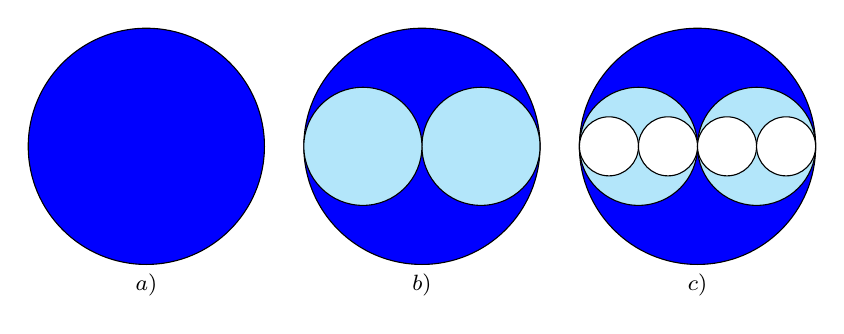
\begin{tikzpicture}[>=stealth,line join=round,line cap=round,font=\footnotesize,scale=1,declare function={r=1.5;}]
\begin{scope}
\draw[fill=blue] (0,0)circle(r);
\path (0,-r) node[below]{$a)$};
\end{scope}
\begin{scope}[xshift={3.5cm}]
\draw[fill=blue] (0,0)circle(r);
\draw[fill=cyan!30] (r/2,0)circle(r/2);
\draw[fill=cyan!30] (-r/2,0)circle(r/2);
\path (0,-r) node[below]{$b)$};
\end{scope}
\begin{scope}[xshift={7cm}]
\draw[fill=blue] (0,0)circle(r);
\draw[fill=cyan!30] (r/2,0)circle(r/2);
\draw[fill=cyan!30] (-r/2,0)circle(r/2);
\foreach \i in {0,1,2,3}
\draw[fill=white,shift={(r/2*\i,0)}] (-3*r/4,0)circle(r/4);
\path (0,-r) node[below]{$c)$};
\end{scope}
\end{tikzpicture}
\end{center}
\loigiai{
Diện tích của các hình tròn trong các lần cắt là
\begin{itemize}
\item Lần thứ 1: $S_1=\pi R^2$.
\item  Lần thứ 2: $S_2=2\cdot \pi \left(\dfrac{R}{2}\right)^2= \dfrac{\pi R^2}{2}$.
\item  Lần thứ 3: $S_2=4\cdot \pi \left(\dfrac{R}{4}\right)^2= \dfrac{\pi R^2}{2^2}$.	
\item $\ldots$
\item Lần thứ $n$: $S_n= \dfrac{\pi R^2}{2^{n-1}}$.
\end{itemize}
Do đó  diện tích các hình tròn lập thành một cấp số nhân lùi vô hạn có số hạng đầu $S_1=\pi R^2$ và công bội $q=\dfrac{1}{2}$ nên tổng diện tích các hình tròn là 
\[ S_1+S_2+\cdots=\dfrac{\pi R^2}{1-\dfrac{1}{2}}=2\pi R^2. \]
}
\end{vd} 

\begin{vd}%[1D3C1-6]%[Dự án đề cương 3 khối NH24-25-Dot 2-Ngô Tất Thành]
\immini{Tam giác mà ba đỉnh của nó là ba trung điểm ba cạnh của tam giác $ABC$ được gọi là \textit{tam giác trung bình} của tam giác $ABC$. Ta xây dựng dãy các tam giác $A_1B_1C_1$, $A_2B_2C_2$, $A_3B_3C_3$, \ldots sao cho $A_1B_1C_1$ là một tam giác giác đều cạnh bằng $3$ và với mỗi số nguyên dương $n\geq 2$, tam giác $A_nB_nC_n$ là tam giác trung bình của tam giác $A_{n-1}B_{n-1}C_{n-1}$. Với mỗi số nguyên dương $n$, kí hiệu $S_n$ tương ứng là diện tích hình tròn ngoại tiếp tam giác $A_nB_nC_n$. Tính tổng $S=S_1+S_2+\cdots+S_n+\cdots$.
}{
\begin{tikzpicture}[scale=1,line join=round, line cap=round,font=\footnotesize]
\coordinate (A) at (0,3);
\coordinate (B) at (-2,0);
\coordinate (C) at (3,0);
\path ($(A)!0.5!(B)$) coordinate (A_1);
\path ($(B)!0.5!(C)$) coordinate (B_1);
\path ($(A)!0.5!(C)$) coordinate (C_1);
\path ($(A_1)!0.5!(B_1)$) coordinate (A_2);
\path ($(B_1)!0.5!(C_1)$) coordinate (B_2);
\path ($(A_1)!0.5!(C_1)$) coordinate (C_2);
\fill[black] ($(A_2)!0.5!(C_2)$) circle (1.5pt);
\fill[black] ($(A_2)!0.5!(B_2)$) circle (1.5pt);
\fill[black] ($(B_2)!0.5!(C_2)$) circle (1.5pt);
\draw[thick](A)--(B)--(C)--cycle (A_1)--(B_1)--(C_1)--cycle (A_2)--(B_2)--(C_2)--cycle;
\foreach \i/\g in {A/90,B/-90,C/-90,A_1/180,B_1/-90,C_1/0,A_2/210,B_2/-30,C_2/90}{\draw[fill=black](\i) circle (1.5pt) ($(\i)+(\g:3mm)$) node[scale=1]{$\i$};}
\end{tikzpicture}
}
\loigiai{
\immini{
Ta có $S_1=\pi\cdot\left(3\cdot\dfrac{\sqrt{3}}{3}\right)^2=3\pi$;\\ $S_2=\pi\cdot\left(\dfrac{3}{2}\cdot\dfrac{\sqrt{3}}{3}\right)^2=\dfrac{3\pi}{4}=\dfrac{1}{4}\cdot S_1$;\\ $S_3=\pi\cdot\left(\dfrac{3}{4}\cdot\dfrac{\sqrt{3}}{3}\right)^2=\dfrac{3\pi}{16}=\dfrac{1}{4}\cdot S_2$\\
Ta có $S_1$; $S_2$; $S_3$;\ldots;$S_n$; \ldots tạo thành cấp số nhân lùi vô hạn với số hạng đầu là $S_1=3\pi$ và công bội $q=\dfrac{1}{4}$.\\
Suy ra $S=S_1+S_2+\cdots+S_n+\cdots=\dfrac{S_n}{1-q}=\dfrac{3\pi}{1-\dfrac{1}{4}}=4\pi$.
}{
\begin{tikzpicture}[scale=1,line join=round, line cap=round,font=\footnotesize]
\coordinate (A) at (0,3);
\coordinate (B) at (-2,0);
\coordinate (C) at (3,0);
\path ($(A)!0.5!(B)$) coordinate (A_1);
\path ($(B)!0.5!(C)$) coordinate (B_1);
\path ($(A)!0.5!(C)$) coordinate (C_1);
\path ($(A_1)!0.5!(B_1)$) coordinate (A_2);
\path ($(B_1)!0.5!(C_1)$) coordinate (B_2);
\path ($(A_1)!0.5!(C_1)$) coordinate (C_2);
\fill[black] ($(A_2)!0.5!(C_2)$) circle (1.5pt);
\fill[black] ($(A_2)!0.5!(B_2)$) circle (1.5pt);
\fill[black] ($(B_2)!0.5!(C_2)$) circle (1.5pt);
\draw[thick](A)--(B)--(C)--cycle (A_1)--(B_1)--(C_1)--cycle (A_2)--(B_2)--(C_2)--cycle;
\foreach \i/\g in {A/90,B/-90,C/-90,A_1/180,B_1/-90,C_1/0,A_2/210,B_2/-30,C_2/90}{\draw[fill=black](\i) circle (1.5pt) ($(\i)+(\g:3mm)$) node[scale=1]{$\i$};}
\end{tikzpicture}
}	
}
\end{vd}
\Closesolutionfile{ans}
\subsection{Bài tập rèn luyện}
\ind{PHẦN I.} \inden{Câu trắc nghiệm nhiều phương án lựa chọn. Mỗi câu hỏi học sinh chỉ chọn một phương án.}\\
\setcounter{ex}{0}
\Opensolutionfile{ans}[ans/1D3-Bai1-TN]
\begin{ex}%[1D3N1-1]%[Dự án đề cương 3 Khối NH24-25-Dot 2- Ngô Tất Thành]
Phát biểu nào sau đây là \textbf{sai}?
\choice 
{$\lim\limits \dfrac{1}{{{2}^{n}}}=0$}
{\True $\lim\limits \left(\dfrac{3}{2}\right)^n=0$}
{$\lim\limits \dfrac{1}{\left( \sqrt{2}\right)^n}=0$}
{$\lim\limits \left( -\dfrac{\sqrt{3}}{2} \right)^n=0$}
\loigiai{
Phát biểu $\lim\limits \left(\dfrac{3}{2}\right)^n=0$ là sai vì $\lim\limits \left(\dfrac{3}{2}\right)^n=+\infty$.
} \end{ex} 
\begin{ex}%[1D3N1-1]%[Dự án đề cương 3 Khối NH24-25-Dot 2- Ngô Tất Thành]
Cho $\lim\limits u_n=a$, $\lim\limits v_n=b$. Phát biểu nào sau đây là \textbf{sai}?
\choice 
{$\lim\limits \left(u_n + v_n\right)=a+b$}
{$\lim\limits \left(u_n-v_n\right)=a-b$} 
{$\lim\limits \left(u_n\cdot v_n\right) =a\cdot b$}
{\True $\lim\limits \dfrac{u_n}{v_n} =\dfrac{a-b}{b}$}
\loigiai{
Phát biểu	$\lim\limits  \dfrac{u_n}{v_n}  =\dfrac{a-b}{b}$ là sai vì $\lim\limits  \dfrac{u_n}{v_n} =\dfrac{a}{b}$.
} \end{ex} 
\begin{ex}%[1D3N1-1]%[Dự án đề cương 3 Khối NH24-25-Dot 2- Ngô Tất Thành]
Nếu $\lim\limits u_n=C$ và $\lim\limits v_n=+\infty $ (hoặc $\lim\limits v_n=-\infty $) thì $\lim\limits \dfrac{u_n}{v_n}$ bằng
\choice 
{\True $0$}
{$-\infty$}
{$+\infty$}
{$-\infty$ hoặc $+\infty$}
\loigiai{
Ta có $\lim\limits \dfrac{u_n}{v_n}=0$.} \end{ex} 
\begin{ex}%[1D3N1-1] %[Dự án đề cương 3 Khối NH24-25-Dot 2- Ngô Tất Thành]
Phát biểu nào sau đây là \textbf{sai}?
\choice 
{Nếu $\lim\limits u_n=+\infty $ và $\lim\limits v_n=C$, $C>0$ thì $\lim\limits \dfrac{u_n}{v_n}=+\infty$} 
{Nếu $\lim\limits u_n=-\infty $ và $\lim\limits v_n=C$, $C<0$ thì $\lim\limits \dfrac{u_n}{v_n}=+\infty$} 
{\True Nếu $\lim\limits u_n=+\infty $ và $\lim\limits v_n=C$, $C<0$ thì $\lim\limits \dfrac{u_n}{v_n}=0$} 
{Nếu $\lim\limits u_n=-\infty $ và $\lim\limits v_n=C$, $C>0$ thì $\lim\limits \dfrac{u_n}{v_n}=-\infty$}
\loigiai{
Nếu $\lim\limits u_n=+\infty $ và $\lim\limits v_n=C$, $C<0$ thì $\lim\limits \dfrac{u_n}{v_n}=-\infty$.} \end{ex} 
\begin{ex}%[1D3N1-1] %[Dự án đề cương 3 Khối NH24-25-Dot 2- Ngô Tất Thành]
Phát biểu nào sau đây là đúng?
\choice 
{Nếu $\lim\limits u_n=a$ thì $\lim\limits \sqrt{u_n}=\sqrt{a}$} 
{Nếu $\lim\limits u_n=a$ thì $a\ge 0$ và $\lim\limits \sqrt{u_n}=\sqrt{a}$} 
{Nếu $\lim\limits u_n=a$ thì $a\ge 0$} 
{\True Nếu $u_n\ge 0$ với mọi $n$ và $\lim\limits u_n=a$ thì $a\ge 0$ và $\lim\limits \sqrt{u_n}=\sqrt{a}$}
\loigiai{
\lq\lq Nếu $u_n\ge 0$ với mọi $n$ và $\lim\limits u_n=a$ thì $a\ge 0$ và $\lim\limits \sqrt{u_n}=\sqrt{a}$\rq\rq là phát biểu đúng.
} \end{ex}

\begin{ex}%[1D3N1-1]%[Dự án đề cương 3 Khối NH24-25-Dot 2- Ngô Tất Thành]
Cho $\lim\limits u_n=2$, $\lim\limits v_n=3$. Khi đó, $\lim\limits \left( u_n+v_n\right) $ bằng 
\choice 
{$6$}
{\True $5$}
{$1$}
{$2$}
\loigiai{
Ta có $\lim\limits \left( u_n+v_n\right)=2+3=5$. 
} \end{ex}

\begin{ex}%[1D3N1-1]%[Dự án đề cương 3 Khối NH24-25-Dot 2- Ngô Tất Thành] 
Cho $\lim\limits u_n=3$, $\lim\limits v_n=+\infty $. Khi đó, $\lim\limits \dfrac{v_n}{u_n}$ bằng
\choice 
{$3$}
{$-\infty $}
{\True $+\infty$}
{$0$}
\loigiai{
Ta có $\lim\limits \dfrac{v_n}{u_n}=+\infty$.} \end{ex} 

\begin{ex}[ĐỀ THI HK1 TRƯỜNG THPT TUY PHONG - BÌNH THUẬN - NĂM HỌC2024-2025] %[1D3N1-1]%[Dự án đề cương 3 Khối NH24-25-Dot 2- Ngô Tất Thành] 
Phát biểu nào sau đây là \textbf{sai}?
\choice
{$\lim\limits q^n=0$ $(|q|<1)$}
{\True $\lim\limits (-2)^n=+\infty$}
{$\lim\limits \dfrac{1}{n}=0$}
{$\lim\limits n=+\infty$}
\loigiai{
Phát biểu \textbf{sai} là $\lim\limits (-2)^n=+\infty$.
}
\end{ex}

\begin{ex}%[1D3H1-2] %[Dự án đề cương 3 Khối NH24-25-Dot 2- Ngô Tất Thành]
Cho hai dãy số với $\left(u_n\right)$, $\left(v_n\right)$ với $u_n=1-\dfrac{2}{n}$, $v_n=4+\dfrac{2}{n+2}$. Khi đó, $\lim\limits \left( u_n+\sqrt{v_n}\right)$ bằng
\choice 
{\True $3$}
{$4$}
{$5$}
{$2$}
\loigiai{
Ta có $\lim\limits u_n=\lim\limits \left( 1-\dfrac{2}{n}\right)=1$, $\lim\limits v_n=\lim\limits \left( 4+\dfrac{2}{n+2}\right)=4$.\\
Vậy $\lim\limits \left( u_n+\sqrt{v_n}\right)=1+\sqrt{4}=3$.
} \end{ex}



\begin{ex}[Đề thi HK1 trường THPT Lê Hồng Phong năm học 2425]%[1D3N1-1]%[Dự án đề cương 3 Khối NH24-25-Dot 2- Ngô Tất Thành]
Cho dãy số $(u_n)$ có $\lim\limits u_n=2$. Tính $\lim\limits\dfrac{2u_n+5}{3u_n-1}$.
\choice
{$\dfrac{2}{3}$}
{$-\dfrac{1}{5}$}
{\True $\dfrac{9}{5}$}
{$+\infty $}
\loigiai
{
Ta có $\lim\limits\dfrac{2u_n+5}{3u_n-1}=\dfrac{2\cdot 2+5}{3\cdot 2-1}=\dfrac{9}{5}$.
}
\end{ex}

\begin{ex}[ĐỀ THI HK1 TRƯỜNG THPT THUẬN THÀNH SỐ 1 - NĂM HỌC 2024-2025]%[1D3H1-2]
Giới hạn $\lim\limits \dfrac{4n+2}{n-1}$ bằng
\choice
{$-2$}
{$2$}
{$-1$}
{\True $4$}
\loigiai{
Ta có $\lim\limits \dfrac{4n+2}{n-1}=\lim\limits \dfrac{4+\dfrac{2}{n}}{1-\dfrac{1}{n}}=4$.
}	
\end{ex}

\begin{ex}[ĐỀ THI HK1 TRƯỜNG VINH KI-NĂM HỌC 2024-2025]%[1D3H1-2]%[Dự án đề cương 3 Khối NH24-25-Dot 2- Ngô Tất Thành]
Giá trị của $\lim\limits \dfrac{3n^2-5n+1}{5+n^2}$ bằng
\choice
{$-1$}
{\True $3$}
{$\dfrac{3}{5}$}
{$+\infty$}
\loigiai{
Ta có $\lim\limits \dfrac{3n^2-5n+1}{5+n^2}=\lim\limits \dfrac{3-\dfrac{5}{n}+\dfrac{1}{n^2}}{1+\dfrac{5}{n^2}}=3$.
}
\end{ex}

\begin{ex}[Đề thi HK1 trường THPT PHẠM PHÚ THỨ năm học 2425]%[1D3H1-2]%[Dự án đề cương 3 Khối NH24-25-Dot 2- Ngô Tất Thành]
Cho dãy số $(u_n)$ với $u_n=\dfrac{2n^2-n}{n^2+1}$. Tính $\lim\limits u_n$.
\choice
{\True$2$}
{$\dfrac{1}{2}$}
{$-1$}
{$1$}
\loigiai{
Ta có $\lim\limits u_n=\lim\limits\dfrac{2n^2-n}{n^2+1}=\lim\limits\dfrac{2-\dfrac{1}{n2}}{1+\dfrac{1}{n^2}}=2$.
}
\end{ex}

\begin{ex}[ĐỀ THI HK1 TRƯỜNG NGUYỄN KHUYẾN - NĂM HỌC 2024-2025]%[1D3H1-2]%[Dự án đề cương 3 Khối NH24-25-Dot 2- Ngô Tất Thành]
Cho $\lim\limits\dfrac{n^2-n+1}{3n^2-4}=\dfrac{a}{b}$, với $\dfrac{a}{b}$ là phân số tối giản. Mệnh đề nào sau đây là đúng?
\choice
{$a+b=2$}
{$a+b=3$}
{\True $a+b=4$}
{$a+b=5$}
\loigiai 
{
Ta có $\lim\limits\dfrac{n^2-n+1}{3n^2-4}=\lim\limits\dfrac{1-\dfrac{1}{n}+\dfrac{1}{n^2}}{3-\dfrac{4}{n^2}}=\dfrac{1}{3}$, suy ra $a=1$ và $b=3$.\\
Vậy $a+b=1+3=4$.
}
\end{ex}

\begin{ex}[ĐỀ THI HK1 LỚP 11 TRƯỜNG THPT TRẦN PHÚ - HCM - NĂM HỌC 2024-2025]%[1D3H1-2]%[Dự án đề cương 3 Khối NH24-25-Dot 2- Ngô Tất Thành]
Giới hạn $\lim\limits \dfrac{3^n - 4^n + 5^n}{3^n + 4^n - 5^n}$ bằng
\choice
{$1$}
{\True $-1$}
{$3$}
{$0$}
\loigiai{
Ta có $\lim\limits \dfrac{3^n - 4^n + 5^n}{3^n + 4^n - 5^n}=\lim\limits\dfrac{\left(\dfrac{3}{5}\right)^n-\left(\dfrac{4}{5}\right)^n+1}{\left(\dfrac{3}{5}\right)^n+\left(\dfrac{4}{5}\right)^n-1}=\dfrac{1}{-1}=-1$.
}
\end{ex}

\begin{ex}%[1D3H1-2]%[Dự án đề cương 3 Khối NH24-25-Dot 2- Ngô Tất Thành]
Tính giới hạn $\lim\limits\dfrac{\sqrt{8 n^{2} + n - 3}}{n - 4}$.
\choice
{ \True $2 \sqrt{2}$}
{ $ 8 $}
{ $- \dfrac{3}{4}$}
{ $ \dfrac{3}{4}$}
\loigiai{ 
Ta có $\lim\limits\dfrac{\sqrt{8 n^{2} + n - 3}}{n - 4}=\lim\limits \dfrac{\sqrt{8+\dfrac{1}{n}-\dfrac{3}{n^2}}}{1-\dfrac{4}{n}}=2\sqrt{2}$.
}\end{ex}

\begin{ex}[ĐỀ THI HK1 SỞ GD\&ĐT BẮC NINH - NĂM HỌC 2024-2025]%[1D3H1-3]%[Dự án đề cương 3 Khối NH24-25-Dot 2- Ngô Tất Thành]
Giới hạn $\lim\limits \left(\sqrt{n^2+4n}-n\right)$ bằng
\choice
{$4$}
{$+\infty$}
{\True $2$}
{$0$}
\loigiai{
Ta có $\lim\limits \left(\sqrt{n^2+4n}-n\right)
=\lim\limits \dfrac{4n}{\sqrt{n^2+4n}+n}
=\lim\limits \dfrac{4}{\sqrt{1+\dfrac{4}{n}}+1}
=\dfrac{4}{2}=2$.
}
\end{ex}

\begin{ex}[ĐỀ THI HK1 SỞ BẮC NINH - NĂM HỌC 2024-2025]%[1D3N1-4]%[Dự án đề cương 3 Khối NH24-25-Dot 2- Ngô Tất Thành]
Giới hạn $\lim\limits \left(2^n+3^n-4^n\right)$ bằng
\choice
{$1$}
{$-4$}
{$+\infty$}
{\True $-\infty$}
\loigiai{
Ta có $\lim\limits \left(2^n+3^n-4^n\right)
=\lim\limits 4^n\left[\left(\dfrac{2}{4}\right)^n+\left(\dfrac{3}{4}\right)^n-1\right]
=-\infty$.\\
Vì $\lim\limits 4^n=+\infty$ và $\lim\limits \left[\left(\dfrac{2}{4}\right)^n+\left(\dfrac{3}{4}\right)^n-1\right]=-1<0$.
}
\end{ex}

\begin{ex}[Đề thi HK1 trường THPT PHẠM PHÚ THỨ - Năm học 2024-2025]%[1D2H3-6]%[Dự án đề cương 3 Khối NH24-25-Dot 2- Ngô Tất Thành]
Tính tổng $T=2+\dfrac{2}{3}+\dfrac{2}{3^2}+\cdots+\dfrac{2}{3^{n-1}}+\cdots$.
\choice
{$4$}
{$6$}
{\True$3$}
{$5$}
\loigiai{
Dãy		$2$; $\dfrac{2}{3}$; $\dfrac{2}{3^2}$; $\dfrac{2}{3^3}$; $\ldots$; $\dfrac{2}{3^{n-1}}$; $\ldots$ là một cấp số nhân lùi vô hạn với số hạng đầu $u_1=2$, công bội $q=\dfrac{1}{3}$.\\
Do đó		$T=2+\dfrac{2}{3}+\dfrac{2}{3^2}+\cdots+\dfrac{2}{3^{n-1}}+\cdots=\dfrac{u_1}{1-q}=\dfrac{2}{1-\dfrac{1}{3}}=3$.
}
\end{ex}

\begin{ex}[Đề thi HK1 - Sở Bắc Ninh - NH 2024-2025]%[1D3H1-5]%[Dự án đề cương 3 Khối NH24-25-Dot 2- Ngô Tất Thành]
Tổng $S=1-\dfrac{1}{3}+\dfrac{1}{3^2}-\dfrac{1}{3^3}+\cdots+\left(-\dfrac{1}{3}\right)^n+\cdots$ bằng
\choice
{$\dfrac{2}{3}$}
{$\dfrac{3}{2}$}
{\True $\dfrac{3}{4}$}
{$\dfrac{4}{3}$}
\loigiai{
Dãy $1$; $-\dfrac{1}{3}$; $\dfrac{1}{3^2}$; $-\dfrac{1}{3^3}$; $\ldots$; $\left(-\dfrac{1}{3}\right)^n$; $\ldots$ là một cấp số nhân lùi vô hạn với số hạng đầu $u_1=1$, công bội $q=-\dfrac{1}{3}$.\\
Do đó $S=\dfrac{u_1}{1-q}=\dfrac{1}{1+\dfrac{1}{3}}=\dfrac{3}{4}$.
}
\end{ex}
\Closesolutionfile{ans}

\ind{PHẦN II.} \inden{Câu trắc nghiệm đúng sai. Trong mỗi ý a), b), c), d) ở mỗi câu, học sinh chọn đúng hoặc sai.}\\
\setcounter{ex}{0}
\Opensolutionfile{ans}[ans/1D3-Bai1-DS]
\begin{ex}%[1D3H1-2]%[Dự án đề cương 3 Khối NH24-25-Dot 2- Ngô Tất Thành]
Cho hai dãy số $\left( u_n\right) $ và $\left( v_n\right)$ có $u_n=n^2 - 4n + 3$, $v_n=- n^2 + 7n - 7$. 
\choiceTF
{ $\lim\limits \dfrac{u_n}{v_n}=- \dfrac{3}{7}$}
{ $\lim\limits \dfrac{u_n}{(v_n)^2}=1$}
{ $\lim\limits \dfrac{u_n}{v_n- 2 n^{2}}=1$}
{ \True Với $m=-4$ thì $\lim\limits \dfrac{u_n+mn^2-5}{v_n-5}=3$}
\loigiai{ 

\begin{itemchoice}
\itemch Ta có:
$\lim\limits \dfrac{u_n}{v_n}=\lim\limits \dfrac{n^2 - 4n + 3}{-n^2 + 7n - 7}
=\lim\limits \dfrac{1 - \dfrac{4}{n} + \dfrac{3}{n^{2}}}{-1 + \dfrac{7}{n} - \dfrac{7}{n^{2}}}=-1$.

\itemch Ta có:
$\lim\limits \dfrac{u_n}{(v_n)^2}=\lim\limits \dfrac{n^{2} - 4 n + 3}{\left(- n^{2} + 7 n - 7\right)^{2}}=\lim\limits \dfrac{n^{2} \cdot \left(1 - \dfrac{4}{n} + \dfrac{3}{n^{2}}\right)}{n^{2} \left(-1 + \dfrac{7}{n} - \dfrac{7}{n^{2}}\right)^{2}}
=\lim\limits \dfrac{1 - \dfrac{4}{n} + \dfrac{3}{n^{2}}}{\left(-1 + \dfrac{7}{n} - \dfrac{7}{n^{2}}\right)^{2}}=0$.

\itemch Ta có:
$\lim\limits \dfrac{u_n}{v_n- 2 n^{2}}=\lim\limits \dfrac{n^{2} - 4 n + 3}{- n^{2} + 7 n - 7- 2 n^{2}} =\lim\limits \dfrac{n^{2} - 4 n + 3}{- 3 n^{2} + 7 n - 7} =\lim\limits \dfrac{1 - \dfrac{4}{n} + \dfrac{3}{n^{2}}}{-3 + \dfrac{7}{n} - \dfrac{7}{n^{2}}}=- \dfrac{1}{3}$.

\itemch Ta có:
$\lim\limits \dfrac{u_n+mn^2+-5}{v_n-5}=3 \Rightarrow \lim\limits \dfrac{n^{2} - 4 n + 3+mn^2-5}{- n^{2} + 7 n - 7-5}=3\Rightarrow \dfrac{1+m}{-1}=3 \Rightarrow m=-4$.
\end{itemchoice}

}\end{ex}

\begin{ex}%[1D3H1-5]%[Dự án đề cương 3 Khối NH24-25-Dot 2- Ngô Tất Thành]
\choiceTF
{ \True  $\lim\limits 51=51$}
{ \True  $\lim\limits \dfrac{4 - 3n}{2n + 1}=- \dfrac{3}{2}$}
{ \True  $\lim\limits \dfrac{\left(- n^{2} - 2\right)^{2}}{5 n^4 + 4n^3 + 3n + 4}=\dfrac{1}{5}$}
{ \True  $S=-1- \dfrac{2}{9}- \dfrac{4}{81}+\cdots+(-1)\cdot\left(\dfrac{2}{9}\right)^{n-1}+\cdots=- \dfrac{9}{7}$}
\loigiai{ 
\begin{itemchoice}
\itemch
$\lim\limits 51=51$.		
\itemch
$\lim\limits \dfrac{4 - 3 n}{2 n + 1}=\lim\limits \dfrac{-3 + \dfrac{4}{n}}{2 + \dfrac{1}{n}}= - \dfrac{3}{2}$.
\itemch
$\lim\limits \dfrac{\left(- n^{2} - 2\right)^{2}}{5 n^{4} + 4 n^{3} + 3 n + 4}=\lim\limits \dfrac{\left(-1 - \dfrac{2}{n^{2}}\right)^{2}}{5 + \dfrac{4}{n} + \dfrac{3}{n^{3}} + \dfrac{4}{n^{4}} }= \dfrac{1}{5}$.
\itemch
Dãy số	$-1$, $-\dfrac{2}{9}$, $-\dfrac{4}{81}$, $\ldots$ lập thành cấp số nhân với $u_1=-1$, $q=\dfrac{2}{9}$.\\
Vậy	$S=-1- \dfrac{2}{9}- \dfrac{4}{81}+\cdots +(-1)\cdot\left(\dfrac{2}{9}\right)^{n-1}+\cdots=\dfrac{-1}{1-\dfrac{2}{9}}=-\dfrac{9}{7}$.
\end{itemchoice}

}\end{ex}

\begin{ex}%[0D0H2-2]%[Dự án đề cương 3 Khối NH24-25-Dot 2- Ngô Tất Thành]
Một bệnh nhân hàng ngày phải uống một viên thuốc $150$\,mg. Sau ngày đầu, trước mỗi lần uống, hàm lượng thuốc cũ trong cơ thể vẫn còn $5$\%.
\choiceTF
{\True Lượng thuốc trong cơ thể bệnh nhân sau khi uống viên thuốc của ngày đầu tiên là $150$\,mg}
{\True Lượng thuốc trong cơ thể bệnh nhân sau khi uống viên thuốc của ngày thứ hai là $150(1+0{,}05)$\,mg}
{Lượng thuốc trong cơ thể bệnh nhân sau khi uống viên thuốc của ngày thứ năm là $160$\,mg}
{\True Lượng thuốc trong cơ thể bệnh nhân nếu bệnh nhân sử dụng thuốc trong một thời gian dài là $\dfrac{400}{361}$\,mg}
\loigiai{
\begin{itemchoice}
\itemch 
Lượng thuốc trong cơ thể bệnh nhân sau khi uống viên thuốc của ngày đầu tiên là $150$ mg.
\itemch 
Sau ngày đầu, trước mỗi lần uống, hàm lượng thuốc cũ trong cơ thể vẫn còn 5\%.\\		
Do đó, lượng thuốc trong cơ thể bệnh nhân sau khi uống viên thuốc của ngày thứ hai là		
$$150 + 150\cdot 5\% = 150(1+0{,}05).$$
\itemch 
Lượng thuốc trong cơ thể bệnh nhân sau khi uống viên thuốc của ngày thứ ba là			
\[150+150(1+0{,}05)\cdot 5\% =150+150(0{,}05+0{,}052)=150(1+0{,}05+0{,}05^2).\]
Lượng thuốc trong cơ thể bệnh nhân sau khi uống viên thuốc của ngày thứ tư là			
\[150+150(1+0{,}05+0{,}052)\cdot5\%=150(1+0{,}05+0{,}05^2+0{,}05^3).\]
Lượng thuốc trong cơ thể bệnh nhân sau khi uống viên thuốc của ngày thứ năm là			
\[150+150(1+0{,}05+0{,}052+0{,}053)\cdot 5\%=150(1+0{,}05+0{,}05^2+0{,}05^3+0{,}05^4)=157{,}8946875\, \mathrm{(mg)}.\]
\itemch 
Ta ước tính lượng thuốc trong cơ thể bệnh nhân nếu bệnh nhân sử dụng thuốc trong một thời gian dài là			
\[S=150\left( 1+0{,}05+0{,}05^2+0{,}05^3+0{,}05^4+\ldots \right) \,\mathrm{(mg)}.\]			
Lại có $1+0{,}05+0{,}05^2+0{,}05^3+0{,}05^4+\ldots$ là tổng của cấp số nhân lùi vô hạn với số hạng đầu $u_1=1$ và công bội $q=0{,}05$.\\			
Do đó, $1+0{,}05+0{,}05^2+0{,}05^3+0{,}05^4+\ldots=\dfrac{u_1}{1-q}=\dfrac{1}{1-0{,}05}=\dfrac{20}{19}$.\\
Suy ra $S=150\cdot \dfrac{20}{19}=\dfrac{400}{361}$\,mg.
\end{itemchoice}
}
\end{ex} 

\begin{ex}%[1D3V1-6]%[Dự án đề cương 3 Khối NH24-25-Dot 2- Ngô Tất Thành]
Từ độ cao $55{,}8$\,m của tháp nghiêng Pisa nước Ý, người ta thả một quả bóng cao su chạm xuống đất. Giả sử mỗi lần chạm đất, quả bóng nảy lên với độ cao bằng $\dfrac{1}{10}$ độ cao mà quả bóng đạt được trước đó. Gọi $h_n$ là độ cao mà của bóng đạt được ở lần nảy thứ $n$.
\choiceTF
{Số hạng tổng quát của dãy số $\left(h_n\right)$ là $\dfrac{55{,}8}{10^{n-1}}$}
{\True Độ cao của của bóng ở lần nảy thứ $3$ bằng $0{,}0558$\,m}
{\True Giới hạn của dãy số $\left(h_n\right)$ bằng $0$}
{\True Tổng quãng đường mà quả bóng di chuyển từ khi thả cho đến khi dừng hẳn (kết quả làm tròn đến hàng phần chục) bằng $68{,}2$\,m}
\begin{center}
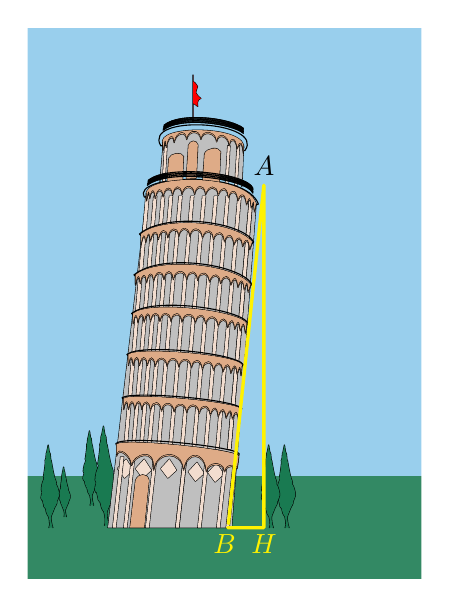
\begin{tikzpicture}[line join=round, line cap=round,scale=1,transform shape]
\definecolor{lightcornflowerblue}{rgb}{0.6, 0.81, 0.93}
\definecolor{cadmiumgreen}{rgb}{0.0, 0.42, 0.24}
\definecolor{trueblue}{rgb}{0.0, 0.45, 0.81}
\definecolor{tumbleweed}{rgb}{0.87, 0.67, 0.53}%màu cát
\clip (-2,-3.5) rectangle (3,3.5);

\tikzset{thap/.pic={%Xây từ dưới lên
\def\T{ 
(-.88,-1.78)%1
..controls +(40:.17) and +(120:.1) ..  (.686,-1.91)--(.68,-1.94)
..controls +(120:.1) and +(40:.12) ..  (-.87,-1.81)
--cycle

(-.8,-1.2)%2
..controls +(40:.14) and +(120:.14) ..  (.72,-1.34)--(.7,-1.36)
..controls +(120:.1) and +(40:.12) ..  (-.78,-1.23)
--cycle

(-.74,-.65)%3
..controls +(40:.22) and +(120:.17) ..  (.74,-.78)--(.72,-.8)
..controls +(120:.15) and +(40:.15) ..  (-.72,-.67)
--cycle

(-.68,-.13)%4
..controls +(40:.34) and +(110:.2) ..  (.8,-.26)--(.78,-.28)
..controls +(110:.17) and +(40:.27) ..  (-.66,-.15)
--cycle

(-.65,.36)%5
..controls +(40:.44) and +(120:.3) ..  (.85,.24)--(.83,.22)
..controls +(130:.35) and +(40:.35) ..  (-.63,.34)
--cycle

(-.58,.88)%6
..controls +(40:.44) and +(120:.3) ..  (.87,.78)--(.85,.76)
..controls +(130:.35) and +(40:.35) ..  (-.56,.86)
--cycle

(-.52,1.35)%7
..controls +(120:.32) and +(110:.47) ..  (.93,1.26)--(.9,1.25)
..controls +(110:.43) and +(110:.27) ..  (-.49,1.35)
--cycle

(-.31,2)%8
..controls +(120:.47) and +(55:.46) ..  (.76,1.94)--(.74,1.94)
..controls +(75:.31) and +(115:.28) ..  (-.28,2)
--cycle

(-.48,1.5)
..controls +(40:.33) and +(110:.2) ..  (.86,1.4)
(-.476,1.52)
..controls +(40:.33) and +(110:.2) ..  (.86,1.42)
(-.472,1.54)
..controls +(40:.33) and +(110:.2) ..  (.86,1.44)
(-.468,1.56)
..controls +(40:.33) and +(110:.2) ..  (.86,1.46)

(-.28,2.2)
..controls +(40:.27) and +(140:.2) ..  (.74,2.16)
(-.276,2.22)
..controls +(40:.27) and +(140:.2) ..  (.74,2.18)
(-.272,2.24)
..controls +(40:.27) and +(140:.2) ..  (.74,2.2)
(-.268,2.26)
..controls +(40:.27) and +(140:.2) ..  (.74,2.22)
;}
\draw \T;
%\fill[tumbleweed] \T;
}}

\tikzset{rao/.pic={%Rào
\def\R{ 
(-.48,1.5)
..controls +(40:.33) and +(110:.2) ..  (.86,1.4)
(-.476,1.52)
..controls +(40:.33) and +(110:.2) ..  (.86,1.42)
(-.472,1.54)
..controls +(40:.33) and +(110:.2) ..  (.86,1.44)
(-.468,1.56)
..controls +(40:.33) and +(110:.2) ..  (.86,1.46)
(-.28,2.2)
..controls +(40:.27) and +(140:.2) ..  (.74,2.16)
(-.276,2.22)
..controls +(40:.27) and +(140:.2) ..  (.74,2.18)
(-.272,2.24)
..controls +(40:.27) and +(140:.2) ..  (.74,2.2)
(-.268,2.26)
..controls +(40:.27) and +(140:.2) ..  (.74,2.22)
;}
\draw \R;
%\fill[tumbleweed] \R;
}}

\tikzset{co/.pic={%Cờ
\def\C{ 
(0.1,2.3)--(.1,2.9)
(.1,2.82)
..controls +(-40:.2) and +(140:.22) ..  (.2,2.6)
..controls +(-60:0) and +(100:.1) ..(.16,2.5)
..controls +(140:.1) and +(-30:0) ..  (.1,2.53)--cycle
;}
\draw \C;
\fill[red] \C;
}}

\tikzset{cong0/.pic={%Đường cong trệt
\def\D0{ 
(.68,-1.96)
..controls +(120:.1) and +(40:.12) ..  (-.87,-1.81)--
(-.87,-1.94)
..controls +(80:.12) and +(95:0.12) ..  (-.68,-2.06)
..controls +(80:.12) and +(85:0.3) ..  (-.4,-2.12)
..controls +(80:.25) and +(95:0.25) ..  (-.02,-2.12)
..controls +(80:.25) and +(95:0.25) ..  (.27,-2.14)
..controls +(80:.12) and +(95:0.12) ..  (.5,-2.14)
..controls +(70:.12) and +(95:0.02) ..  (.66,-2.1)--cycle
;}
\draw \D0;
\fill[tumbleweed] \D0;
}}

\tikzset{cong1/.pic={%Đường cong 1
\def\D1{ 
(.7,-1.36)
..controls +(120:.1) and +(40:.12) ..  (-.78,-1.23)--
(-.78,-1.35)
..controls +(80:.12) and +(95:0.12) ..  (-.72,-1.35)
..controls +(80:.12) and +(95:0.12) ..  (-.64,-1.35)
..controls +(80:.12) and +(95:0.12) ..  (-.55,-1.35)
..controls +(80:.12) and +(95:0.12) ..  (-.44,-1.36)
..controls +(80:.12) and +(95:0.12) ..  (-.3,-1.37)
..controls +(80:.12) and +(95:0.12) ..  (-.14,-1.38)
..controls +(80:.12) and +(95:0.12) ..  (0.02,-1.39)
..controls +(80:.12) and +(95:0.12) ..  (0.18,-1.4)
..controls +(80:.12) and +(95:0.12) ..  (0.32,-1.42)
..controls +(70:.12) and +(95:0.12) ..  (0.42,-1.44)
..controls +(70:.12) and +(95:0.12) ..  (0.52,-1.46)
..controls +(70:.12) and +(95:0.12) ..  (0.6,-1.47)
..controls +(70:.12) and +(95:0.12) ..  (0.68,-1.5)--cycle
;}
\draw \D1;
\fill[tumbleweed] \D1;
}}

\tikzset{cong2/.pic={%Đường cong 2
\def\D2{ 
(.72,-.8)
..controls +(120:.15) and +(40:.15) ..  (-.72,-.67)--
(-.72,-.79)
..controls +(80:.12) and +(95:0.12) ..  (-.66,-.79)
..controls +(80:.12) and +(95:0.12) ..  (-.58,-.79)
..controls +(80:.12) and +(95:0.12) ..  (-.48,-.79)
..controls +(80:.12) and +(95:0.12) ..  (-.38,-.8)
..controls +(80:.12) and +(95:0.12) ..  (-.23,-.8)
..controls +(80:.12) and +(95:0.12) ..  (-0.08,-.81)
..controls +(80:.12) and +(95:0.12) ..  (0.08,-.82)
..controls +(80:.12) and +(95:0.12) ..  (0.22,-.84)
..controls +(80:.12) and +(95:0.12) ..  (0.36,-.85)
..controls +(70:.12) and +(95:0.12) ..  (0.48,-.87)
..controls +(70:.12) and +(95:0.12) ..  (0.58,-.89)
..controls +(70:.12) and +(95:0.12) ..  (0.66,-.9)
..controls +(70:.12) and +(95:0.12) ..  (0.71,-.92)--cycle
;}
\draw \D2;
\fill[tumbleweed] \D2;
}}

\tikzset{cong3/.pic={%Đường cong 3
\def\D3{ 
(.78,-.28)
..controls +(110:.17) and +(40:.27) ..  (-.66,-.15)--
(-.66,-.26)
..controls +(80:.12) and +(95:0.12) ..  (-.6,-.25)
..controls +(80:.12) and +(95:0.12) ..  (-.52,-.24)
..controls +(80:.12) and +(95:0.12) ..  (-.44,-.23)
..controls +(80:.12) and +(95:0.12) ..  (-.32,-.23)
..controls +(80:.12) and +(95:0.12) ..  (-.18,-.23)
..controls +(80:.12) and +(95:0.12) ..  (-.04,-.24)
..controls +(80:.12) and +(95:0.12) ..  (0.13,-.25)
..controls +(80:.12) and +(95:0.12) ..  (0.26,-.26)
..controls +(70:.12) and +(95:0.12) ..  (0.42,-.29)
..controls +(70:.12) and +(95:0.12) ..  (0.54,-.31)
..controls +(70:.12) and +(95:0.12) ..  (0.63,-.33)
..controls +(70:.12) and +(95:0.12) ..  (0.7,-.35)
..controls +(70:.12) and +(95:0.12) ..  (0.765,-.38)--cycle
;}
\draw \D3;
\fill[tumbleweed] \D3;
}}

\tikzset{cong4/.pic={%Đường cong 4
\def\D4{ 
(.83,.22)
..controls +(130:.35) and +(40:.35) ..  (-.63,.34)--
(-.63,.23)
..controls +(80:.12) and +(95:0.12) ..  (-.57,.25)
..controls +(80:.12) and +(95:0.12) ..  (-.49,.26)
..controls +(80:.12) and +(95:0.12) ..  (-.4,.28)
..controls +(80:.12) and +(95:0.12) ..  (-.27,.3)
..controls +(80:.12) and +(95:0.12) ..  (-.15,.3)
..controls +(80:.12) and +(95:0.12) ..  (0.02,.3)
..controls +(80:.12) and +(95:0.12) ..  (0.16,.29)
..controls +(80:.12) and +(95:0.12) ..  (0.31,.27)
..controls +(70:.12) and +(95:0.12) ..  (0.45,.25)
..controls +(70:.12) and +(95:0.12) ..  (0.58,.23)
..controls +(70:.12) and +(95:0.12) ..  (0.67,.2)
..controls +(70:.12) and +(95:0.12) ..  (0.75,.17)
..controls +(70:.12) and +(95:0.12) ..  (0.8,.14)--cycle
;}
\draw \D4;
\fill[tumbleweed] \D4;
}}

\tikzset{cong5/.pic={%Đường cong 5
\def\D5{ 
(.85,.76)
..controls +(130:.35) and +(40:.35) ..  (-.56,.86)--
(-.56,.74)
..controls +(80:.12) and +(95:0.12) ..  (-.5,.77)
..controls +(80:.12) and +(95:0.12) ..  (-.44,.79)
..controls +(80:.12) and +(95:0.12) ..  (-.34,.81)
..controls +(80:.12) and +(95:0.12) ..  (-.22,.83)
..controls +(80:.12) and +(95:0.12) ..  (-0.08,.85)
..controls +(80:.12) and +(95:0.12) ..  (0.06,.85)
..controls +(80:.12) and +(95:0.12) ..  (0.22,.83)
..controls +(70:.12) and +(95:0.12) ..  (0.36,.81)
..controls +(70:.12) and +(95:0.12) ..  (0.5,.78)
..controls +(70:.12) and +(95:0.12) ..  (0.62,.74)
..controls +(70:.12) and +(95:0.12) ..  (0.73,.72)
..controls +(70:.12) and +(95:0.12) ..  (0.82,.68)--cycle
;}
\draw \D5;
\fill[tumbleweed] \D5;
}}

\tikzset{cong6/.pic={%Đường cong 6
\def\D6{ 
(.9,1.25)
..controls +(110:.43) and +(110:.27) ..  (-.49,1.35)--
(-.49,1.3)
..controls +(80:.12) and +(95:0.12) ..  (-.45,1.33)
..controls +(80:.12) and +(95:0.12) ..  (-.38,1.33)
..controls +(80:.12) and +(95:0.12) ..  (-.28,1.35)
..controls +(80:.12) and +(95:0.12) ..  (-.16,1.37)
..controls +(80:.12) and +(95:0.12) ..  (-0.04,1.38)
..controls +(80:.12) and +(95:0.12) ..  (0.12,1.38)
..controls +(80:.12) and +(95:0.12) ..  (0.26,1.38)
..controls +(70:.12) and +(95:0.12) ..  (0.42,1.37)
..controls +(70:.12) and +(95:0.12) ..  (0.55,1.34)
..controls +(70:.12) and +(95:0.12) ..  (0.67,1.3)
..controls +(70:.12) and +(95:0.12) ..  (0.78,1.25)
..controls +(70:.12) and +(95:0.12) ..  (0.84,1.21)
..controls +(70:.12) and +(95:0.12) ..  (0.88,1.16)--cycle
;}
\draw \D6;
\fill[tumbleweed] \D6;
}}

\tikzset{cong7/.pic={%Đường cong 7
\def\D7{ 
(.74,1.94)
..controls +(75:.31) and +(115:.28) ..  (-.28,2)--
(-.28,1.94)
..controls +(80:.12) and +(95:0.12) ..  (-.24,1.98)
..controls +(80:.12) and +(95:0.12) ..  (-.14,2.04)
..controls +(80:.12) and +(95:0.12) ..  (0.02,2.08)
..controls +(80:.12) and +(95:0.12) ..  (0.2,2.08)
..controls +(80:.12) and +(95:0.12) ..  (0.4,2.05)
..controls +(80:.12) and +(95:0.12) ..  (0.56,2)
..controls +(80:.12) and +(95:0.12) ..  (0.66,1.96)
..controls +(70:.12) and +(95:0.12) ..  (0.74,1.9)--cycle
;}
\draw \D7;
\fill[tumbleweed] \D7;
}}

\tikzset{cua/.pic={%Cửa
\def\W{ 
(-.7,-2.85)--(-.63,-2.25)
..controls +(70:.1) and +(100:.1) ..  (-.46,-2.25)--(-.52,-2.85)
--cycle
;}
\draw \W;
\fill[tumbleweed] \W;
}}

\tikzset{vien/.pic={%viền ngoài
\def\V{ 
(.9,1.25)
..controls +(110:.43) and +(110:.27) ..  (-.49,1.35)--(-.98,-2.85)--(.59,-2.85)--cycle

(.74,1.94)
..controls +(75:.31) and +(115:.28) ..  (-.28,2)--(-.32,1.54)
..controls +(115:.2) and +(75:.13) ..  (.72,1.48)--cycle
;}
\draw \V;
\fill[gray!50!] \V;
}}

\tikzset{soc/.pic={%Thanh sọc
\def\S{ 
(.82,1.36)--(.54,-1.85)--(.58,-1.85)--(.86,1.36)
--cycle
;}
\draw \S;
\fill[tumbleweed!40!] \S;
}}

\tikzset{soc2/.pic={%Thanh sọc lớn
\def\S{ 
(.54,-1.95)--(.44,-2.85)--(.48,-2.85)--(.58,-1.95)
--cycle
;}
\draw \S;
\fill[tumbleweed!40!] \S;
}}

\tikzset{soc3/.pic={%Thanh sọc
\def\S{ 
(.54,2)--(.57,2)--(.54,1.5)--(.51,1.5)
--cycle
(.66,2)--(.69,2)--(.66,1.5)--(.63,1.5)
--cycle
(-.26,2)--(-.23,2)--(-.26,1.5)--(-.29,1.5)
--cycle
;}
\draw \S;
\fill[tumbleweed!40!] \S;
}}

\tikzset{thoi/.pic={%Hình thoi
\def\T{ 
(0.15,-1.98)--(.24,-2.12)--(0.13,-2.22)--(0.04,-2.1)
--cycle
;}
\draw \T;
\fill[tumbleweed!40!] \T;
}}

\tikzset{cay/.pic={%Cây
\def\T{ 
(-1.73,-2.85)
..controls +(40:.03) and +(40:.01) ..  (-1.74,-2.7)
..controls +(140:.04) and +(60:.02) ..  (-1.78,-2.6)
..controls +(140:.04) and +(60:.02) ..  (-1.8,-2.55)
..controls +(100:.03) and +(70:.02) ..  (-1.82,-2.5)
..controls +(140:.04) and +(60:.02) ..  (-1.815,-2.4)
..controls +(140:.04) and +(60:.02) ..  (-1.818,-2.3)
..controls +(85:.03) and +(-30:.03) ..  (-1.8,-2.2)
..controls +(80:.04) and +(50:.02) ..  (-1.78,-2)
..controls +(60:.04) and +(120:.02) ..  (-1.76,-1.9)
..controls +(80:.03) and +(-100:.02) ..  (-1.74,-1.8)
..controls +(80:.01) and +(-100:.02) ..  (-1.72,-1.9)
..controls +(60:.02) and +(-120:.02) ..  (-1.7,-2)
..controls +(-80:.02) and +(110:.03) ..  (-1.66,-2.2)
..controls +(-100:.02) and +(60:.03) ..  (-1.64,-2.3)
..controls +(-30:.02) and +(70:.02) ..  (-1.6,-2.44)
..controls +(-100:.02) and +(70:.02) ..  (-1.63,-2.52)
..controls +(-60:.02) and +(70:.01) ..  (-1.66,-2.6)
..controls +(60:.01) and +(70:.02) ..  (-1.7,-2.7)
..controls +(-120:.02) and +(120:.03) ..  (-1.68,-2.85)
;}
\draw \T;
\fill[cadmiumgreen!90!] \T;
}}
\fill[cadmiumgreen!80!] (-4,-3.5) rectangle (8,-2.2);
\fill[lightcornflowerblue] (-4,3.5) rectangle (8,-2.2);
\path 
(0,0)pic[scale=1]{cay}(.35,0)pic[scale=.9]{cay}(1.05,0.6)pic[scale=1.2]{cay}(-.5,-1)pic[scale=.6]{cay}
(3,0)pic[scale=1]{cay}(2.8,0)pic[scale=1]{cay}
(0,0)pic[scale=1]{vien}
(0,0)pic[scale=1]{soc} (0,0)pic[scale=1]{soc}(-.15,0)pic[scale=1]{soc}(-.3,0)pic[scale=1]{soc}(-.45,0)pic[scale=1]{soc}(-.6,0)pic[scale=1]{soc}(-.75,0)pic[scale=1]{soc}(-.9,0)pic[scale=1]{soc}(-1.02,0)pic[scale=1]{soc}(-1.12,0)pic[scale=1]{soc}(-1.22,0)pic[scale=1]{soc}(-1.32,0)pic[scale=1]{soc}

(0,0)pic[scale=1]{soc3}
(0,0)pic[scale=1]{thap}(0,0)pic[scale=1]{co}
(.4,3.6)pic[scale=.7,rotate=3]{cua}
(.8,3.6)pic[scale=1.2,rotate=7,yscale=.6]{cua}
(.3,3.4)pic[scale=1.1,rotate=7,yscale=.6]{cua}
(0,-.04)pic[scale=1]{thoi}(0.25,-.05)pic[scale=1]{thoi}(-0.35,0)pic[scale=1]{thoi}(-.67,0)pic[scale=1]{thoi}(-.9,0)pic[scale=1]{thoi}
(-1.22,0)pic[scale=1]{soc2}(-1.36,0)pic[scale=1]{soc2}
(-.94,0)pic[scale=1]{soc2}(-.56,0)pic[scale=1]{soc2}
(-.56,0)pic[scale=1]{soc2}(.08,0)pic[scale=1]{soc2}(-.04,0)pic[scale=1]{soc2}(-.28,0)pic[scale=1]{soc2}
(0,0)pic[scale=1]{cong0} (0,0.02)pic[scale=1]{cong0}%
(0,0)pic[scale=1]{cong1} (0,0.02)pic[scale=1]{cong1}%
(0,0)pic[scale=1]{cong2} (0,0.02)pic[scale=1]{cong2}%
(0,0)pic[scale=1]{cong3}(0,0.02)pic[scale=1]{cong3}
(0,0)pic[scale=1]{cong4}(0,0.02)pic[scale=1]{cong4}
(0,0)pic[scale=1]{cong5}(0,0.02)pic[scale=1]{cong5}
(0,0)pic[scale=1]{cong6}(0,0.02)pic[scale=1]{cong6}
(0,0)pic[scale=1]{cong7}(0,0.02)pic[scale=1]{cong7}
(0,0)pic[scale=1]{cua}
(0,0)pic[scale=1]{rao}
;
\draw [color=yellow,line width=1.2pt](0.55,-2.8)--(1,1.5)--++(0,-4.35)--++(-0.46,0);
\draw [color=yellow,line width=1.2pt] (0.5,-2.8)node[below]{$B$};
\draw [color=yellow,line width=1.2pt] (1,-2.8)node[below]{$H$};
\draw (1,1.5)node[above]{$A$};
\end{tikzpicture}
\end{center}
\loigiai{
Quả bóng rơi từ độ cao ban đầu $h=55{,}8$\,m.\\
Độ cao nảy lên lần lượt là $h_1=\dfrac{1}{10}\cdot h$, $h_2=\dfrac{1}{10}\cdot h_1$,\dots .\\
Dãy $h_1$, $h_2$, $h_3$,\dots là cấp số nhân với công bội $q=\dfrac{1}{10}$ và số hạng đầu $h_1=\dfrac{1}{10}\cdot55{,}8=5{,}58$.\\

\begin{itemchoice}
\itemch
Số hạng tổng quát của dãy số là $\left(h_n\right)$ là $h_n=h_1\cdot q=5{,}58\cdot \left( \dfrac{1}{10}\right)^{n-1}= \dfrac{55{,}8}{10^n}$.
\itemch
Ta có $h_3= \dfrac{55{,}8}{10^3}=0{,}0558$\,m.
\itemch
Ta có $\lim\limits h_n=\lim\limits \dfrac{55{,}8}{10^n} =0$.
\itemch
Tổng quãng đường quả bóng di chuyển đến khi dừng hẳn bằng $S=h+2(h_1+h_2+h_3+\dots)$.\\ Ta có tổng cấp số nhân vô hạn
$h_1+h_2+h_3+\dots=\dfrac{h_1}{1-q}=\dfrac{5{,}58}{1-\dfrac{1}{10}}=6{,}2$\,m.\\
Vậy $S=55{,}8+2\cdot6{,}2=55{,}8+12{,}4=68{,}2$\,m.
\end{itemchoice}
}
\end{ex}

\begin{ex}[Đề HK1 trường THPT thị xã Quảng Trị, Quảng Trị, năm học 2024-2025]%[1D2V3-8]%[Dự án đề cương 3 Khối NH24-25-Dot 2- Ngô Tất Thành]
Cho hình vuông $(C_1)$ có cạnh bằng $3$. Người ta chia mỗi cạnh của hình vuông thành bốn phần bằng nhau và nối các điểm chia một cách thích hợp để có hình vuông $(C_2)$ (tham khảo hình vẽ minh họa).
\begin{center}
\begin{tikzpicture}[scale=0.9, font=\footnotesize, line join=round, line cap=round, >=stealth]
\def\a{3}
\def\j{7}
\draw (\a,\a) coordinate(A1)--
(-\a,\a) coordinate(B1)--
(-\a,-\a) coordinate(C1)--
(\a,-\a) coordinate(D1)--cycle;
\foreach \i [count=\k from 2] in {1,2,...,\j} \draw ($(A\i)!0.25!(B\i)$) coordinate(A\k)--
($(B\i)!0.25!(C\i)$) coordinate(B\k)--	
($(C\i)!0.25!(D\i)$) coordinate(C\k)--
($(D\i)!0.25!(A\i)$) coordinate(D\k)--
cycle;
\end{tikzpicture}
\end{center}
Từ hình vuông $(C_2)$ tiếp tục làm như trên ta nhận được dãy các hình vuông $(C_1)$, $(C_2)$, $(C_3)$, \ldots, $(C_n)$, \ldots. Gọi $S_i$ là diện tích hình vuông $(C_i)$ với $i\in \{1,2,3,\ldots\}$, $T=S_1+S_2+S_3+ \cdots +S_n+ \cdots$.
\choiceTF
{\True Diện tích  hình vuông $\left( C_3\right) $ là $\dfrac{225}{64}$}
{Số hạng tổng quát của dãy số $\left( S_n\right) $ là $S_n=9\cdot \left(\dfrac{5}{8}\right)^n$}
{Giới hạn của dãy số $\left( S_n\right) $ bằng $+\infty$}
{\True $T=24$} 
\loigiai
{Giả sử $a_i$ là cạnh hình vuông $\left(C_i\right)$ ($i\in \{1,2,\ldots\}$).\\
Ta có $a_1=3$, hình vuông thứ $(C_{i+1})$ có cạnh bằng cạnh huyền của tam giác vuông với một cạnh tam giác bằng $\dfrac{1}{4}$ cạnh hình vuông $(C_i)$ và cạnh còn lại bằng $\dfrac{3}{4}$ cạnh hình vuông $(C_i)$.\\
Do đó $a_{i+1}= \sqrt{\left(\dfrac{a_i}{4}\right)^2 + \left(\dfrac{3a_i}{4}\right)^2} =\sqrt{\dfrac{a_i^2}{16} + \dfrac{9a_i^2}{16}} = \sqrt{\dfrac{5}{8}a_i^2}$.\\
Vì vậy $S_1=a_1^2=9$, $S_{i+1}=a_{i+1}^2 = \dfrac{5}{8}a_i^2 = \dfrac{5}{8}S_i$ với mọi $i\in \mathbb{N}^*$.\\
Suy ra $(S_n)$ lập thành cấp số nhân với $S_1=9$, công bội $q=\dfrac{5}{8}$.\\
\begin{itemchoice}
\itemch
Diện tích  hình vuông $\left( C_3\right)$ là $S_3=\dfrac{5}{8}S_2=\dfrac{5}{8}\dfrac{5}{8}S_1=\dfrac{225}{64}$.
\itemch Vì vậy $S_1=a_1^2=9$, $S_{i+1}=a_{i+1}^2 = \dfrac{5}{8}a_i^2 = \dfrac{5}{8}S_i$ với mọi $i\in \mathbb{N}^*$.\\
Suy ra $(S_n)$ lập thành cấp số nhân với $S_1=9$, công bội $q=\dfrac{5}{8}$.\\
Số hạng tổng quát $S_n=S_1\cdot \left( \dfrac{5}{8}\right)^{n-1}=9\cdot\left( \dfrac{5}{8}\right)^{n-1}$.
\itemch $\lim\limits S_n=\lim\limits \left( 9\cdot\left( \dfrac{5}{8}\right)^{n-1}\right)  =0$.

\itemch	
Ta có $T=S_1+S_2+ \cdots + S_n + \cdots$ là tổng của cấp số nhân lùi vô hạn với $S_1=9$, $q=\dfrac{5}{8}$.\\
Vậy $T=S_1+S_2+ \cdots + S_n + \cdots = \dfrac{S_1}{1-q} = \dfrac{9}{1-\dfrac{5}{8}} = 24$.
\end{itemchoice}

}
\end{ex}
\Closesolutionfile{ans}
\ind{PHẦN III.} \inden{Câu trắc nghiệm trả lời ngắn.}\\
\Opensolutionfile{ans}[ans/1D3-Bai1-KQ]
\setcounter{ex}{0}
%%%=============EX_1=============%%%
\begin{ex}%[1D3V1-3]%[Dự án đề cương 3 khối NH24-25-Dot 2-Ngô Tất Thành]
Tính $\lim\limits\left(\sqrt{n^2+2n}-n\right)$.
\par \shortans[oly]{1}
\loigiai{
\allowdisplaybreaks
\begin{eqnarray*}
\lim\limits\left(\sqrt{n^2+2n}-n\right)&=&\lim\limits\dfrac{\left(\sqrt{n^2+2n}-n\right)\left(\sqrt{n^2+2n}+n\right)}{\sqrt{n^2+2n}+n}\\
&=&\lim\limits \dfrac{n^2+2n-n^2}{\sqrt{n^2+2n}+n}\\
&=&\lim\limits \dfrac{2n}{\sqrt{n^2+2n}+n}\\
&=&\lim\limits \dfrac{2}{\sqrt{1+\dfrac{2}{n}}+1}\\
&=&1.
\end{eqnarray*}
}
\end{ex}


%%%=============EX_2=============%%%
\begin{ex}%[1D3V1-3]%[Dự án đề cương 3 khối NH24-25-Dot 2-Ngô Tất Thành]
Biết $\lim\limits \dfrac{n-\sqrt{2n^2+1}}{4+3n}=\dfrac{a-\sqrt{b}}{c}$ (biết $a$, $b$, $c$ là các số nguyên dương). Tính $a^2 +b^2 +c^2$.
\par \shortans[oly]{14}
\loigiai
{
$\lim\limits \dfrac{n-\sqrt{2n^2+1}}{4+3n}
= \lim\limits \dfrac{n \left(1- \sqrt{2+\tfrac{1}{n^2}}\right)}{n \left(3+ \tfrac{4}{n} \right)}
= \lim\limits \dfrac{1- \sqrt{2+\tfrac{1}{n^2}}}{3+ \tfrac{4}{n} }
= \dfrac{1-\sqrt{2}}{3}
$. \\
Do đó, $a=1$, $b=2$, $c=3$ $\Rightarrow a^2 +b^2 +c^2 = 14$.
}
\end{ex}


%%%=============EX_3=============%%%
\begin{ex}%[1D3V1-3]%[Dự án đề cương 3 khối NH24-25-Dot 2-Ngô Tất Thành]
	Biết rằng $$\lim\limits\left(\sqrt[3]{n^3+3}-\sqrt{n^2+2}\right)=\lim\limits\dfrac{a}{\sqrt[3]{\left(n^3+3\right)^2}+n^2+n\cdot \sqrt[3]{n^3+3}}-\lim\limits\dfrac{b}{n+\sqrt{n^2+2}}$$ với $a;b$ là các số nguyên dương. Tính $T=2a+3b$.
\par \shortans[oly]{$12$}
	\loigiai{
		Ta có \begin{eqnarray*}
			\lim\limits\left(\sqrt[3]{n^3+3}-\sqrt{n^2+2}\right)&=&\lim\limits\left(\sqrt[3]{n^3+3}-n\right)+\lim\limits\left(n-\sqrt{n^2+2}\right)\\
			&=&\lim\limits\dfrac{n^3+3-n^3}{\left(n^3+3\right)^{\tfrac{2}{3}}+n^2+n\cdot \sqrt[3]{n^3+3}}+\lim\limits\dfrac{n^2-n^2-2}{n+\sqrt{n^2+2}}\\
			&=&\lim\limits\dfrac{3}{\left(n^3+3\right)^{\tfrac{2}{3}}+n^2+n\cdot \sqrt[3]{n^3+3}}-\lim\limits\dfrac{2}{n+\sqrt{n^2+2}}\\
			&=&\lim\limits\dfrac{3}{\sqrt[3]{\left(n^3+3\right)^2}+n^2+n\cdot \sqrt[3]{n^3+3}}-\lim\limits\dfrac{2}{n+\sqrt{n^2+2}}.
		\end{eqnarray*}
		Do đó $a=3$; $b=2$ và $2a+3b=12$.
	}
\end{ex}


%%%=============EX_4=============%%%
\begin{ex}[Đề CKI - THPT Vàm Đình 2024-25 - Cà Mau]%[1D3V1-4]%[Dự án đề cương 3 khối NH24-25-Dot 2-Ngô Tất Thành]
Một hình vuông màu vàng có cạnh $1$ đơn vị dài được chia thành chín hình vuông nhỏ hơn và hình vuông ở chính giữa được tô màu xanh như hình vẽ bên dưới. Mỗi hình vuông màu vàng nhỏ hơn lại được chia thành chín hình vuông con, và mỗi hình vuông con ở chính giữa lại được tô màu xanh. Nếu quá trình này được tiếp tục lặp lại năm lần, thì tổng diện tích các hình vuông được tô màu xanh bao nhiêu? (kết quả làm tròn đến hàng phần trăm).
\begin{center}
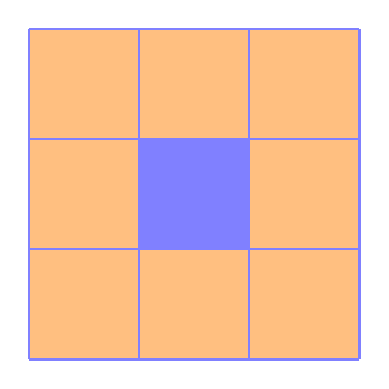
\begin{tikzpicture}[>=stealth,thick,scale=0.7]
\def\n{1}
\def\a{3}
\pgfmathsetmacro{\m}{int(3^(\n))}
\def\hv#1{
\ifnum#1>0
\fill[blue!50] (-\a/3,-\a/3) rectangle (\a/3,\a/3);
\pgfmathtruncatemacro{\k}{#1-1}
\foreach \i in {0,...,3}{
\begin{scope}[shift={(90*\i:2)},scale=1/3]
\hv{\k}
\end{scope}
}
\foreach \i in {0,...,3}{
\begin{scope}[shift={(45+90*\i:{4/sqrt(2)})},scale=1/3]
\hv{\k}
\end{scope}
}
\fi
}
\fill[orange!50] (-\a,-\a) rectangle (\a,\a);
\hv{\n}
\foreach \i in {0,1,...,\m}{
\draw[blue!50]
({-\a+2*\i *\a/\m},\a)--++(270:2*\a)
(\a,{-\a+2*\i *\a/\m})--++(180:2*\a)
;
}
\end{tikzpicture}
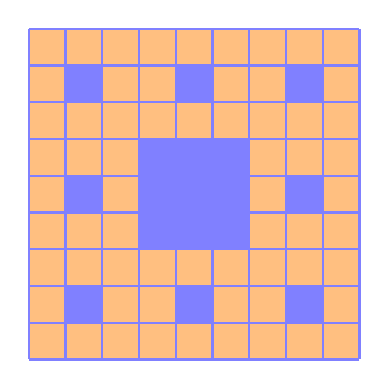
\begin{tikzpicture}[>=stealth,thick,scale=0.7]
\def\n{2}
\def\a{3}
\pgfmathsetmacro{\m}{int(3^(\n))}
\def\hv#1{
\ifnum#1>0
\fill[blue!50] (-\a/3,-\a/3) rectangle (\a/3,\a/3);
\pgfmathtruncatemacro{\k}{#1-1}
\foreach \i in {0,...,3}{
\begin{scope}[shift={(90*\i:2)},scale=1/3]
\hv{\k}
\end{scope}
}
\foreach \i in {0,...,3}{
\begin{scope}[shift={(45+90*\i:{4/sqrt(2)})},scale=1/3]
\hv{\k}
\end{scope}
}
\fi
}
\fill[orange!50] (-\a,-\a) rectangle (\a,\a);
\hv{\n}
\foreach \i in {0,1,...,\m}{
\draw[blue!50]
({-\a+2*\i *\a/\m},\a)--++(270:2*\a)
(\a,{-\a+2*\i *\a/\m})--++(180:2*\a)
;
}
\end{tikzpicture}
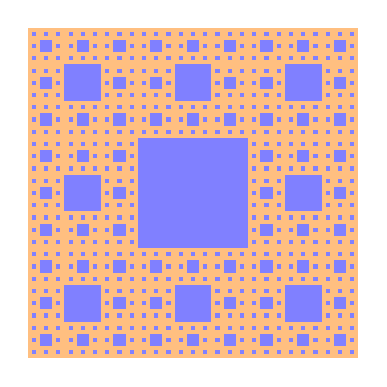
\begin{tikzpicture}[>=stealth,thick,scale=0.7]
\def\n{4}
\def\a{3}
\def\hv#1{
\ifnum#1>0
\fill[blue!50] (-\a/3,-\a/3) rectangle (\a/3,\a/3);
\pgfmathtruncatemacro{\k}{#1-1}
\foreach \i in {0,...,3}{
\begin{scope}[shift={(90*\i:2)},scale=1/3]
\hv{\k}
\end{scope}
}
\foreach \i in {0,...,3}{
\begin{scope}[shift={(45+90*\i:{4/sqrt(2)})},scale=1/3]
\hv{\k}
\end{scope}
}
\fi
}
\fill[orange!50] (-\a,-\a) rectangle (\a,\a);
\hv{\n}
\end{tikzpicture}
\end{center}
\par \shortans[oly]{0{,}45}
\loigiai{
Diện tích ô vuông màu xanh sau lần phân chia thứ nhất là $\dfrac{1}{9}$, số ô vuông màu xanh được tạo thêm là ${{8}^{0}}.$\\
Diện tích ô vuông màu xanh sau lần phân chia thứ hai là $\dfrac{1}{{{9}^{2}}}$, số ô vuông màu xanh được tạo thêm là ${{8}^{1}} \ldots$\\
Diện tích ô vuông màu xanh sau lần phân chia thứ năm là $\dfrac{1}{{{9}^{5}}}$, số ô vuông màu xanh được tạo thêm là ${{8}^{4}}.$\\
Tổng diện tích các ô vuông màu xanh là  $$\dfrac{1}{9}+\dfrac{1}{{{9}^{2}}}\cdot {{8}^{1}}+\ldots +\dfrac{1}{{{9}^{5}}}\cdot {{8}^{4}}\approx 0{,}45.$$
}
\end{ex}

%%%=============EX_5=============%%%
\begin{ex}[Đề CKI - THPT Chu Văn An - An Giang]%[1D3V1-5]%[Dự án đề cương 3 khối NH24-25-Dot 2-Ngô Tất Thành]
Lục giác mà sáu đỉnh của nó là sáu trung điểm sáu cạnh của lục giác $ABCDEF$ được gọi là \textbf{lục giác trung bình} của lục giác $ABCDEF$. Bạn An từ nhỏ đã rất thích hình học, nên khi được bố xây lại phòng, An đã xin bố tự thiết kế cửa sổ của mình như hình vẽ. Trong đó, An đã tạo ra dãy các
lục giác đều $A_{1}B_{1}C_{1}D_{1}E_{1}F_{1}$, $A_{2}B_{2}C_{2}D_{2}E_{2}F_{2}$, $A_{3}B_{3}C_{3}D_{3}E_{3}F_{3}$,$\ldots$ sao cho $A_{1}B_{1}C_{1}D_{1}E_{1}F_{1}$ là lục giác đều
cạnh bằng $1$(m) và với mỗi số nguyên dương $n \ge 2$, lục giác $A_{n}B_{n}C_{n}D_{n}E_{n}F_{n}$ là lục giác trung bình của lục giác $A_{n-1}B_{n-1}C_{n-1}D_{n-1}E_{n-1}F_{n-1}$. Ngoài ra, với mỗi lục giác An lại dựng thêm đường tròn ngoại tiếp lục giác đó. Cửa sổ bao gồm các cạnh của các lục giác và các đường tròn đều được làm
bằng thép. Tính độ dài đoạn thép Bạn An cần sử dụng để trang trí? (kết quả làm tròn đến hàng đơn vị).
\begin{center}
\begin{tikzpicture}[line join=round, line cap=round,>=stealth,font=\footnotesize,scale=1]
\def\a{3.3}
\path 	(0:0) coordinate (O)
%Vẽ lục giác chỉ số 1
(O)++(60:\a) coordinate (A_1)
(O)++(0:\a) coordinate (B_1)
(O)++(-60:\a) coordinate (C_1)
(O)++(-120:\a) coordinate (D_1)
(O)++(180:\a) coordinate (E_1)
(O)++(-240:\a) coordinate (F_1)
%Vẽ lục giác chỉ số 2
($(A_1)!0.5!(B_1)$) coordinate (A_2)
($(B_1)!0.5!(C_1)$) coordinate (B_2)
($(C_1)!0.5!(D_1)$) coordinate (C_2)
($(D_1)!0.5!(E_1)$) coordinate (D_2)
($(E_1)!0.5!(F_1)$) coordinate (E_2)
($(F_1)!0.5!(A_1)$) coordinate (F_2)
%Vẽ lục giác chỉ số 3
($(A_2)!0.5!(B_2)$) coordinate (A_3)
($(B_2)!0.5!(C_2)$) coordinate (B_3)
($(C_2)!0.5!(D_2)$) coordinate (C_3)
($(D_2)!0.5!(E_2)$) coordinate (D_3)
($(E_2)!0.5!(F_2)$) coordinate (E_3)
($(F_2)!0.5!(A_2)$) coordinate (F_3)
%Vẽ lục giác chỉ số 4
($(A_3)!0.5!(B_3)$) coordinate (A_4)
($(B_3)!0.5!(C_3)$) coordinate (B_4)
($(C_3)!0.5!(D_3)$) coordinate (C_4)
($(D_3)!0.5!(E_3)$) coordinate (D_4)
($(E_3)!0.5!(F_3)$) coordinate (E_4)
($(F_3)!0.5!(A_3)$) coordinate (F_4)
%Vẽ lục giác chỉ số 5
($(A_4)!0.5!(B_4)$) coordinate (A_5)
($(B_4)!0.5!(C_4)$) coordinate (B_5)
($(C_4)!0.5!(D_4)$) coordinate (C_5)
($(D_4)!0.5!(E_4)$) coordinate (D_5)
($(E_4)!0.5!(F_4)$) coordinate (E_5)
($(F_4)!0.5!(A_4)$) coordinate (F_5)
%Vẽ lục giác chỉ số 5
($(A_4)!0.5!(B_4)$) coordinate (A_5)
($(B_4)!0.5!(C_4)$) coordinate (B_5)
($(C_4)!0.5!(D_4)$) coordinate (C_5)
($(D_4)!0.5!(E_4)$) coordinate (D_5)
($(E_4)!0.5!(F_4)$) coordinate (E_5)
($(F_4)!0.5!(A_4)$) coordinate (F_5)
%Vẽ lục giác chỉ số 6
($(A_5)!0.5!(B_5)$) coordinate (A_6)
($(B_5)!0.5!(C_5)$) coordinate (B_6)
($(C_5)!0.5!(D_5)$) coordinate (C_6)
($(D_5)!0.5!(E_5)$) coordinate (D_6)
($(E_5)!0.5!(F_5)$) coordinate (E_6)
($(F_5)!0.5!(A_5)$) coordinate (F_6)
%Vẽ lục giác chỉ số 7
($(A_6)!0.5!(B_6)$) coordinate (A_7)
($(B_6)!0.5!(C_6)$) coordinate (B_7)
($(C_6)!0.5!(D_6)$) coordinate (C_7)
($(D_6)!0.5!(E_6)$) coordinate (D_7)
($(E_6)!0.5!(F_6)$) coordinate (E_7)
($(F_6)!0.5!(A_6)$) coordinate (F_7)
%Vẽ lục giác chỉ số 8
($(A_7)!0.5!(B_7)$) coordinate (A_8)
($(B_7)!0.5!(C_7)$) coordinate (B_8)
($(C_7)!0.5!(D_7)$) coordinate (C_8)
($(D_7)!0.5!(E_7)$) coordinate (D_8)
($(E_7)!0.5!(F_7)$) coordinate (E_8)
($(F_7)!0.5!(A_7)$) coordinate (F_8)
%Vẽ lục giác chỉ số 9
($(A_8)!0.5!(B_8)$) coordinate (A_9)
($(B_8)!0.5!(C_8)$) coordinate (B_9)
($(C_8)!0.5!(D_8)$) coordinate (C_9)
($(D_8)!0.5!(E_8)$) coordinate (D_9)
($(E_8)!0.5!(F_8)$) coordinate (E_9)
($(F_8)!0.5!(A_8)$) coordinate (F_9)
;
\draw[smooth,thick] (O) circle (\a);
\draw[smooth,thick](O) let \p1=($(O)-(A_2)$) in circle ({veclen(\x1,\y1)});
\draw[smooth,thick](O) let \p1=($(O)-(A_3)$) in circle ({veclen(\x1,\y1)});
\draw[smooth,thick](O) let \p1=($(O)-(A_4)$) in circle ({veclen(\x1,\y1)});
\draw[smooth,thick](O) let \p1=($(O)-(A_4)$) in circle ({veclen(\x1,\y1)});
\draw[smooth,thick](O) let \p1=($(O)-(A_5)$) in circle ({veclen(\x1,\y1)});
\draw[smooth,thick](O) let \p1=($(O)-(A_6)$) in circle ({veclen(\x1,\y1)});
\draw[smooth,thick](O) let \p1=($(O)-(A_7)$) in circle ({veclen(\x1,\y1)});
\draw[smooth,thick](O) let \p1=($(O)-(A_8)$) in circle ({veclen(\x1,\y1)});
\draw[smooth,thick](O) let \p1=($(O)-(A_9)$) in circle ({veclen(\x1,\y1)});
\draw[smooth,thick] (A_1)--(B_1)--(C_1)--(D_1)--(E_1)--(F_1)--(A_1);
\draw[smooth,thick] (A_2)--(B_2)--(C_2)--(D_2)--(E_2)--(F_2)--(A_2);
\draw[smooth,thick] (A_3)--(B_3)--(C_3)--(D_3)--(E_3)--(F_3)--(A_3);
\draw[smooth,thick] (A_4)--(B_4)--(C_4)--(D_4)--(E_4)--(F_4)--(A_4);
\draw[smooth,thick] (A_5)--(B_5)--(C_5)--(D_5)--(E_5)--(F_5)--(A_5);
\draw[smooth,thick] (A_6)--(B_6)--(C_6)--(D_6)--(E_6)--(F_6)--(A_6);
\draw[smooth,thick] (A_7)--(B_7)--(C_7)--(D_7)--(E_7)--(F_7)--(A_7);
\draw[smooth,thick] (A_8)--(B_8)--(C_8)--(D_8)--(E_8)--(F_8)--(A_8);
\draw[smooth,thick] (A_9)--(B_9)--(C_9)--(D_9)--(E_9)--(F_9)--(A_9);
\foreach \x/\g in {O/-90,A_1/30,B_1/0,C_1/-40,D_1/-130,E_1/180,F_1/120,A_2/50,B_2/0,C_2/-40,D_2/-130,E_2/180,F_2/90}
\fill[black] (\x) circle (1pt) ($(\g:3mm)+(\x)$) node {$\x$};
\end{tikzpicture}
\end{center}
\par \shortans[oly]{92}
\loigiai{Với $n=1$, độ dài cạnh và bán kính đường tròn ngoại tiếp lục giác $A_{1}B_{1}C_{1}D_{1}E_{1}F_{1}$ là $1\; \text{(m)}$.\\
Với $n=2$, độ dài cạnh và bán kính đường tròn ngoại tiếp lục giác $A_{2}B_{2}C_{2}D_{2}E_{2}F_{2}$ là $\dfrac{\sqrt{3}}{2}\; \text{(m)}$.\\
Với $n=3$, độ dài cạnh và bán kính đường tròn ngoại tiếp lục giác $A_{3}B_{3}C_{3}D_{3}E_{3}F_{3}$ là $\dfrac{3}{4}\; \text{(m)}$.\\
Với $n=4$, độ dài cạnh và bán kính đường tròn ngoại tiếp lục giác $A_{4}B_{4}C_{4}D_{4}E_{4}F_{4}$ là $\dfrac{3\sqrt{3}}{8}\; \text{(m)}$.\\
...\\
Sử dụng quy nạp, với $n \ge 1$, ta chứng minh được độ dài cạnh và bán kính đường tròn ngoại tiếp lục giác $A_{n}B_{n}C_{n}D_{n}E_{n}F_{n}$ là $\left(\dfrac{\sqrt{3}}{2}\right)^{n-1}\; \text{(m)}$.\\
Với $n \ge 1$, chu vi của lục giác $A_{n}B_{n}C_{n}D_{n}E_{n}F_{n}$ là $6 \cdot \left(\dfrac{\sqrt{3}}{2}\right)^{n-1}\; \text{(m)}$.\\
Tổng chu vi của các lục giác bạn An làm cửa sổ là
$$P_1= 6 \cdot \left(1+\left(\dfrac{\sqrt{3}}{2}\right)+\left(\dfrac{\sqrt{3}}{2}\right)^2+ \ldots \right) = 6 \cdot \dfrac{1}{1-\dfrac{\sqrt{3}}{2}}=24+12\sqrt{3}\; \text{(m)}.$$
Với $n \ge 1$, chu vi đường tròn ngoại tiếp lục giác $A_{n}B_{n}C_{n}D_{n}E_{n}F_{n}$ là 2$\pi \cdot \left(\dfrac{\sqrt{3}}{2}\right)^{n-1}\; \text{(m)}$.\\
Tổng chu vi của các đường tròn để bạn An làm cửa sổ là
$$P_2= 2 \pi \cdot \left(1+\left(\dfrac{\sqrt{3}}{2}\right)+\left(\dfrac{\sqrt{3}}{2}\right)^2+ \ldots \right) = 2 \pi \cdot \dfrac{1}{1-\dfrac{\sqrt{3}}{2}}=\pi \left(8+4\sqrt{3}\right)\; \text{(m)}.$$
Độ dài đoạn thép Bạn An cần sử dụng để trang trí là $$P_1+P_2=24+12\sqrt{3}+\pi \left(8+4\sqrt{3}\right) \approx 92 \; \text{(m)}.$$
}
\end{ex}
\Closesolutionfile{ans}
\ind{PHẦN IV.} \inden{Tự luận.}\\
\Opensolutionfile{ans}[ans/1D3-Bai1-TL]
\setcounterref{ex}{0}
%%%=============BT_1=============%%%
\begin{ex}%[1D3N1-2]%[Dự án đề cương 3 khối NH24-25-Dot 2-Ngô Tất Thành]
Tìm $\lim\limits \dfrac{{n+5}}{3n+2}$.
\loigiai{
Ta có $\lim\limits \dfrac{{n+5}}{3n+2}=\lim\limits \dfrac{1+\dfrac{5}{n}}{3+\dfrac{2}{n}}=\dfrac{1}{3}$.

}
\end{ex}
%%%=============BT_2=============%%%
\begin{ex}%[1D3N1-2]%[Dự án đề cương 3 khối NH24-25-Dot 2-Ngô Tất Thành]
Tính giới hạn: $\lim\limits \left(5-\dfrac{2}{n^3} \right)$.
\loigiai{
Ta có $\lim\limits \left(5-\dfrac{2}{n^3} \right)=5-0=5$.
}
\end{ex}
%%%=============BT_3=============%%%
\begin{ex}%[1D3N1-5]%[Dự án đề cương 3 khối NH24-25-Dot 2-Ngô Tất Thành]
Tìm $\lim\limits \left( {1+\dfrac{1}{2}+\dfrac{1}{4}+\cdots+\dfrac{1}{2^n}}\right) $.
\loigiai{Đặt $u_n=1+\dfrac{1}{2}+\dfrac{1}{4}+\cdots+\dfrac{1}{2^n}$.\\
$u_n$ là tổng của một cấp số nhân lùi vô hạn với $u_1=1$, công bội $q=\dfrac{1}{2}$. \\
Ta có $\lim\limits \left( {1+\dfrac{1}{2}+\dfrac{1}{4}+\cdots+\dfrac{1}{2^n}}\right)= \dfrac{1}{1-\dfrac{1}{2}}=2$.
}
\end{ex}
%%%=============BT_4=============%%%
\begin{ex}%[1D3H1-4]%[Dự án đề cương 3 khối NH24-25-Dot 2-Ngô Tất Thành]
Tính $\lim\limits \left(-2 n^{3}+3 n-1\right)$.
\loigiai{Ta có
$\lim\limits \left(-2 n^{3}+3 n-1\right)=\lim\limits \left[ n^{3}\left(-2+\dfrac{3}{n^{2}}-\dfrac{1}{n^{3}}\right)\right] =-\infty$.\\
(vì $\lim\limits n^{3}=+\infty $;\  $\lim\limits \left(-2+\dfrac{3}{n^{2}}-\dfrac{1}{n^{3}}\right)=-2<0$).
}
\end{ex}
%%%=============BT_5=============%%%
\begin{ex}%[1D3H1-2]%[Dự án đề cương 3 khối NH24-25-Dot 2-Ngô Tất Thành]
Tìm $\lim\limits \dfrac{3^n - 2 \cdot 5^n}{7 + 3 \cdot 5^n}$.
\loigiai{
Ta có
$\lim\limits \dfrac{3^n - 2 \cdot 5^n}{7 + 3 \cdot 5^n} = \lim\limits \dfrac{\left(\dfrac{3}{5}\right)^n - 2}{7 \cdot \left(\dfrac{1}{5}\right)^n + 3} = -\dfrac{2}{3}$.
}
\end{ex}
%%%=============BT_6=============%%%
\begin{ex}%[1D3H1-2]%[Dự án đề cương 3 khối NH24-25-Dot 2-Ngô Tất Thành]
Tìm $\lim\limits\dfrac{\pi ^n+3^n+2^{2n}}{3\pi ^n-3^n+2^{2n+2}}$.
\loigiai{
Ta có
$\lim\limits\dfrac{\pi ^n+3^n+2^{2n}}{3\pi ^n-3^n+2^{2n+2}}=\lim\limits\dfrac{\left(\dfrac{\pi}{4}\right)^n+\left(\dfrac{3}{4}\right)^n+1}{3\cdot\left(\dfrac{\pi}{4}\right)^n-\left(\dfrac{3}{4}\right)^n+2^2}=\dfrac{1}{4}$.
}
\end{ex}
%%%=============BT_7=============%%%
\begin{ex}%[1D3V1-3]%[Dự án đề cương 3 khối NH24-25-Dot 2-Ngô Tất Thành]
Tìm giới hạn của dãy số $(u_n)$ biết $u_n=\sqrt{4n^2+3n}-2n$.
\loigiai{
Ta có
\allowdisplaybreaks
\begin{eqnarray*}
&\lim\limits u_n &=\lim\limits\left(\sqrt{4n^2+3n}-2n\right)\\
&&=\lim\limits\dfrac{4n^2+3n-4n^2}{\sqrt{4n^2+3n}+2n} \\
&&=\lim\limits\dfrac{3n}{n\left(\sqrt{4+\dfrac{3}{n}}+2\right)} \\
&&=\lim\limits\dfrac{3}{\sqrt{4+\dfrac{3}{n}}+2} \\
&&=\dfrac{3}{\sqrt{4+0}+2} \\
&&=\dfrac{3}{4}.
\end{eqnarray*}
Vậy giới hạn của dãy số $(u_n)$ là $\dfrac{3}{4}$.
}
\end{ex}
%%%=============BT_8=============%%%
\begin{ex}%[Đề CKI - THPT Nguyễn Thị Minh Khai - TPHCM]%[1D3V1-4]%[Dự án đề cương 3 khối NH24-25-Dot 2-Ngô Tất Thành]
Tính giới hạn $\lim\limits \left(\sqrt{4n^2+n}-2\,024n \right)$.
\loigiai{
Ta có $\lim\limits \left(\sqrt{4n^2+n}-2\,024n \right)=\lim\limits\left[ n\cdot \left( \sqrt{4+\dfrac{1}{n}}-2\,024 \right) \right]$.\\
Vì $\heva{&\lim\limits n =+\infty\\
&\lim\limits \left( \sqrt{4+\dfrac{1}{n}} -2\,024 \right)=-2\,022 <0 }$ nên $\lim\limits\left[ n\cdot \left( \sqrt{4+\dfrac{1}{n}}-2\,024 \right) \right] =-\infty$.\\
Vậy $\lim\limits \left(\sqrt{4n^2+n}-2\,024n \right)=-\infty$.
}
\end{ex}
%%%=============BT_9=============%%%
\begin{ex}%[1D3V1-6]%[Dự án đề cương 3 khối NH24-25-Dot 2-Ngô Tất Thành]
Người ta làm lỗ thông gió của một ngôi nhà bằng cách ghép một dãy hình tròn có cùng bán kính là $3$\,cm. Kí hiệu $u_n$ là tổng diện tích hình tròn ghép được ở bước thứ $n$. Tìm $n$ nhỏ nhất để $u_n$ vượt quá $9\pi$\,m$^2$.
\begin{center}
\begin{tikzpicture}[scale=0.8]
\shade[top color=gray!15, bottom color=gray!85] (0,0) rectangle (1,1);
\filldraw[fill=white] (0.5,0.5) circle (0.3);
\node at (0.5,-0.5) {Bước 1};
\shade[top color=gray!15, bottom color=gray!85] (3,0) rectangle (5,2);
\foreach \i in {0,1} {
\foreach \j in {0,1} {
\filldraw[fill=white] (\i+3.5,\j+0.5) circle (0.3);
}
}
\node at (4,-0.5) {Bước 2};
\shade[top color=gray!15, bottom color=gray!85] (7,0) rectangle (10,3);
\foreach \i in {0,1,2} {
\foreach \j in {0,1,2} {
\filldraw[fill=white] (\i+7.5,\j+0.5) circle (0.3);
}
}
\node at (8.5,-0.5) {Bước 3};
\shade[top color=gray!15, bottom color=gray!85] (12,0) rectangle (18,6);
\foreach \i in {0,1,2,3} {
\filldraw[fill=white] (\i+12.5,0.5) circle (0.3);
}
\node at (16.5,0.5) {$\dots$};
\node at (14.5,-0.5) {Bước ... Bước $n$};
\end{tikzpicture}
\end{center}
\loigiai{
Ta có
\[
u_1 = \pi \cdot 3^2, \quad u_2 = 4 \cdot \pi \cdot 3^2, \quad u_3 = 9 \cdot \pi \cdot 3^2, \quad \ldots, \quad u_n = n^2 \cdot \pi \cdot 3^2
\]
Xét $u_n > 90\,000 \pi \Rightarrow n^2 > 10\,000 \Rightarrow n > 100$.	\\
Vậy $n = 101$ là giá trị nhỏ nhất để $u_n$ vượt quá $90\,000\pi$.
}
\end{ex}
%%%=============BT_10=============%%%
\begin{ex}[Đề CKI - THPT Thăng Long - TPHCM]%[1D3V1-6]%[Dự án đề cương 3 khối NH24-25-Dot 2-Ngô Tất Thành]
Từ độ cao $63$ m của tháp nghiêng Pi-sa ở Italia, người ta thả một quả bóng cao su xuống đất. Giả sử mỗi lần chạm đất quả bóng lại nảy lên độ cao bằng $\dfrac{1}{10}$ độ cao mà quả bóng đạt được ngay trước đó. Tính độ dài hành trình của quả bóng từ thời điểm ban đầu cho đến khi nó nằm yên trên mặt đất.
\loigiai{
Ta thấy:
Ban đầu bóng cao $63$ m nên chạm đất lần $1$ bóng di chuyển quãng đường $S_1=63~(\mathrm{m})$.\\
Từ lúc chạm đất lần một đến chạm đất lần hai bóng di chuyển được quãng đường là $$S_2=2\left(S_1 \cdot \dfrac{1}{10}\right)=2 \cdot  \left(63 \cdot \dfrac{1}{10}\right)=\dfrac{63}{5}$$ (do độ cao lần hai bằng $\dfrac{1}{10}$ độ cao ban đầu).\\
Từ lúc chạm đất lần hai đến chạm đất lần ba bóng di chuyển được quãng đường là $S_3=S_2 \dfrac{1}{10}$ (do độ cao lần ba bằng $\dfrac{1}{10}$ độ cao lần hai). \\
Cứ tiếp tục như vậy kéo dài ra vô hạn thì ta có được tổng quãng đường mà bóng cao su đã di chuyển là
\allowdisplaybreaks
\begin{eqnarray*}
S&=&S_{1}+S_{2}+S_{3}+\cdots\\&=&S_{1}+S_{2}+S_{2} \cdot \dfrac{1}{10}+S_{2} \cdot\left(\dfrac{1}{10}\right)^{2}+\cdots\\&=&S_{1}+\dfrac{S_{2}}{1-\dfrac{1}{10}}=\dfrac{63}{5} \cdot \dfrac{10}{9}=77~(\mathrm{m}).
\end{eqnarray*}
Vậy quãng đường di chuyển của bóng là $77$ m.
}
\end{ex}
\Closesolutionfile{ans}

